% ---------------------------------------------------------------------
% This document compiles with pdflatex and is made with Koma-Script. 
%
% The Template is based on the template of Michael
% von Riegen, riegen@informatik.uni-hamburg.de, and
% modified at some points
% ---------------------------------------------------------------------
\documentclass[11pt, DIV=10, BCOR=20mm, bibliography=totoc, listof=totoc]{scrbook}

% Import of packages and options that refer to the whole document can be found in myPreamble.sty
\usepackage{myPreamble}
\newacronym{uhi}{UHI}{Urban Heat Island}
\newacronym{buhi}{BUHI}{Boundary Layer Urban Heat Island}
\newacronym{cuhi}{CUHI}{Canopy Urban Heat Island}
\newacronym{suhi}{SUHI}{Surface Urban Heat Islands}
\newacronym{uhii}{UHII}{urban heat island intensity}
\newacronym{rmse}{RMSE}{root mean squared error}
\newacronym{mse}{MSE}{mean squared error}
\newacronym{lst}{LST}{Land Surface Temperatures}
\newacronym{ta}{T$_{air}$}{air temperature}
\newacronym{r2}{R$^2$}{R-squared}
\newacronym{hgb}{HistGB}{Histogram-based Gradient Boosting}
\newacronym{modis}{MODIS}{Moderate Resolution Imaging Spectroradiometer}
\newacronym{dwd}{DWD}{German Weather Service}
\newacronym{wmo}{WMO}{World Meteorological Organization}
\newacronym{pws}{PWS}{private weather station}
\newacronym{cws}{CWS}{citizen weather station}
\newacronym{qc}{QC}{quality control}
\newacronym{eumetnet}{EUMETNET}{European Meteorological Network}
\newacronym{ml}{ML}{machine learning}
\newacronym{pbl}{PBL}{planetary boundary layer}
\newacronym{lcz}{LCZ}{local climate zone}
\newacronym{p2p}{P2P}{peer-to-peer}
\newacronym{sane}{SANE}{Smart Networks for Urban Citizen Participation}
\newacronym{wsn}{WSN}{Wireless sensor networks}
\newacronym{lcs}{LCS}{low-cost sensors}
\newacronym{pm}{PM}{particulate matter}
\newacronym{svf}{SVF}{sky-view factor}
\newacronym{ux}{UX}{user experience}
\newacronym{idw}{IDW}{inverse-distance weighting}
\newacronym{ok}{OK}{Ordinary Kriging}
\newacronym{ai}{AI}{artificial intelligence}
\newacronym{dl}{DL}{deep learning}
\newacronym{ann}{ANN}{Artificial Neural Network}
\newacronym{nan}{NaN}{not a number}
\newacronym{knn}{KNN}{K-Nearest Neighbours}
\newacronym{rf}{RF}{Random Forests}
\newacronym{qrf}{QRF}{Quantile Regression Forests}
\newacronym{svm}{SVM}{Support Vector Machine}
\newacronym{rfsp}{RFsp}{Random Forest for Spatial Predictions Framework}
\newacronym{rfsi}{RFSI}{Random Forest for Spatial Interpolation}
\newacronym{svr}{SVR}{Support Vector Regression}
\newacronym{rbf}{RBF}{Radial Basis Function}
\newacronym{wow}{WOW}{Weather Observations Website}
\newacronym{gee}{Google EE}{Google Earth Engine}
\newacronym{ecv}{ECV}{Essential Climate Variables}
\newacronym{ndvi}{NDVI}{Difference Vegetation Index}
\newacronym{vif}{VIF}{variance inflation factor}

% useful if writing everything in one chapter
%has no affection on input-commands
% \includeonly{kapitel1}

\begin{document}

	% titlepage

	% roman page numbering
	\frontmatter
	
		\begin{titlepage}
	
	% Avoid error "destination with the same identifier" 
	\setcounter{page}{-1}
	
	% Titlepage
	\begin{figure}[h]
		\begin{minipage}[b]{62mm}
			
\includegraphics[width=62mm]{images/unilogo}
		\end{minipage}
		\hspace{4cm}
		%\begin{minipage}[b]{59mm}
		%	\includegraphics[width=59mm]{images/minlogo}
		%\end{minipage}
	\end{figure}
	
	\vfill
	
	\begin{center}
		% TODO Art der Abschlussarbeit 
		\noindent { \huge
			Bachelorarbeit \\
		}
		\vspace{14mm}
		% TODO Title
		\noindent \textbf{\huge
			Titel
		}
		\vspace{60mm}	
	\end{center}
	
	\vfill
	
	% TODO Angaben
	\noindent \textbf{Max Peter Mustermann} \\
	\noindent \rule{\textwidth}{0.4mm} 
	\noindent{\textrm{max.peter.mustermann@informatik.uni-hamburg.de}} \\
	\noindent{\textrm{Studiengang Informatik}} \\
	\noindent{\textrm{Matr.-Nr. 12345678}} \\
	\begin{tabbing}
		\hspace{8em} \=  \kill
		Erstgutachter: \> Professor A. Ersthelfer \\
		Zweitgutachter: \> Professor Z. Eswirdschonwerden \\
		~ \\
		Abgabe: 09.2020
	\end{tabbing}
	
	% Titlepage back
	\newpage 
	\thispagestyle{empty}
	\setcounter{page}{0}
	
	% wenn man Lust auf ein Zitat hat...
	% ... ansonsten auskommentieren
	%~\\ \vfill \noindent 
	%A distributed system is one where the failure of some \\
	%computer I've never heard of can keep me from getting my work done. \\
	%\textit{-- Leslie Lamport}
\end{titlepage}


	\cleardoubleemptypage
	\chapter*{Abstract}
Lorem ipsum dolor sit amet, consectetuer adipiscing elit. Integer quis lectus eget purus auctor sollicitudin. Sed tempus, leo quis nonummy iaculis, tellus justo bibendum mi, eu facilisis est sapien non eros. Ut tincidunt. Proin eleifend tristique est. Nulla facilisi. Cras ante mauris, facilisis at, fringilla quis, venenatis ornare, libero. Nam viverra varius nibh. Suspendisse potenti. Sed velit quam, euismod quis, sagittis eu, sodales sit amet, dui. Sed sed diam. Vivamus tincidunt quam a eros. Ut quis metus. Lorem ipsum dolor sit amet, consectetuer adipiscing elit. Cum sociis natoque penatibus et magnis dis parturient montes, nascetur ridiculus mus. Sed ut tortor. Vestibulum ante ipsum primis in faucibus orci luctus et ultrices posuere cubilia Curae; Curabitur vulputate nibh a tortor. Nullam scelerisque risus nonummy urna tempor sagittis.
	
	% lists (table of contents, list of figures, tables, abbreviations)
	\tableofcontents
	\listoffigures
	\listoftables
	\printglossary
	\printglossary[title=List of Abbreviations,type=\acronymtype]

	% arabic page numbering
	\mainmatter
	
	% Introduction
	% -----------------------------------------------------------------------
% -----------------------------------------------------------------------

\chapter{Introduction}

 Lorem ipsum dolor sit amet, consectetuer\footnote{Hier ist eine Fußnote!} adipiscing elit. Integer quis lectus eget purus auctor sollicitudin. Sed tempus, leo quis nonummy iaculis, tellus justo bibendum mi, eu facilisis est sapien non eros. Ut tincidunt. Proin eleifend tristique est. Nulla facilisi. Cras ante mauris, facilisis at, fringilla quis, venenatis ornare, libero. Nam viverra varius nibh. Suspendisse potenti. Sed velit quam, euismod quis, sagittis eu, sodales sit amet, dui. Sed sed diam. Vivamus tincidunt quam a eros. Ut quis metus. Lorem ipsum dolor sit amet, consectetuer adipiscing elit. Cum sociis natoque penatibus et magnis dis parturient montes, nascetur ridiculus mus. Sed ut tortor. Vestibulum ante ipsum primis in faucibus orci luctus et ultrices posuere cubilia Curae; Curabitur vulputate nibh a tortor. Nullam scelerisque risus nonummy urna tempor sagittis.

\noindent A Listing \ref{lst:soap}.

\begin{center}
	\begin{lstlisting}[caption={SOAP Anfrage an einen HalloWelt-Web-Service},label=lst:soap,language=XML,label={lst:soap}]
		<?xml version='1.0' encoding='UTF-8'>
		<SOAP-ENV:Envelope (*@\label{lst:soapEnv}@*)
		xmlns:SOAP-ENV="http://schemas.xmlsoap.org/soap/envelope/"
		xmlns:xsi="http://www.w3.org/2001/XMLSchema-instance"
		xmlns:xsd="http://www.w3.org/2001/XMLSchema"
		xmlns:ns1="http://localhost/wsdl/HalloWeltService.wsdl">
		
		<SOAP-ENV:Body>(*@\label{lst:soapBody}@*)
		<ns1:gruss>
		<name xsi:type="xsd:string">
		Michael
		</name>
		</ns1:gruss>
		</SOAP-ENV:Body>
		
		</SOAP-ENV:Envelope>
	\end{lstlisting}
\end{center}

Donec tincidunt. Cras tempus purus et quam. Duis semper. Vestibulum eu ligula. Ut non odio. Ut posuere ligula fringilla neque. Cras sodales justo eu massa. Nullam mauris nulla, fermentum et, fringilla sed, imperdiet vitae, turpis. In vehicula fermentum neque. Cum sociis natoque penatibus et magnis dis parturient montes, nascetur ridiculus mus. Quisque orci. Nunc odio. Nam consectetuer egestas augue.

\noindent A complex table:

\begin{table}[h]
	\caption[Transaktionale Ablaufmodelle im Vergleich]{Transaktionale Ablaufmodelle im Vergleich; teilweise aus \cite{DBLP:books/infix/Schwarz99}; das Wort "`Transaktion"' wird in der Tabelle als TA abgekürzt}
	\label{tab:tamodelleVergleich}
	\centering
	\begin{tabular*}{\textwidth}{| l@{\extracolsep\fill} r || c | c | c || c | c || c || c || c | c | c || c | c |}
		\hline
		
		Modelle & 
		\rotatebox{90}{Eigenschaften} &
		\rotatebox{90}{vital} &
		\rotatebox{90}{non-vital} &
		\rotatebox{90}{Alternativtransaktion } &				
		\rotatebox{90}{sequenziell} &
		\rotatebox{90}{parallel} &
		\rotatebox{90}{unabhängig} &
		\rotatebox{90}{temporal} &
		\rotatebox{90}{geschlossen geschachtelt } &
		\rotatebox{90}{offen geschachtelt} &
		\rotatebox{90}{Kompensation} &
		\rotatebox{90}{endliche Schachtelung } &
		\rotatebox{90}{unendliche Schachtelung } \\
		
		\hline
		\hline
		
		\multicolumn{2}{|l||}{Geschl. gesch. TA} &
		\checkmark &
		(\checkmark) &
		(\checkmark) &
		\checkmark &
		\checkmark &
		
		- &
		- &
		
		\checkmark &
		- &
		-	&
		\checkmark &
		\checkmark \\
		\hline
		
		\multicolumn{2}{|l||}{Offen gesch. TA} &
		\checkmark &
		(\checkmark) &
		(\checkmark) &
		\checkmark &
		\checkmark &
		
		- &
		- &
		
		- &
		\checkmark &
		\checkmark &
		\checkmark &
		\checkmark \\
		\hline
		
		\multicolumn{2}{|l||}{Sagas} &
		\checkmark &
		- &
		- &
		\checkmark &
		- &
		
		- &
		- &
		
		- &
		\checkmark &
		\checkmark &	
		\checkmark &
		- \\
		\hline
		
		\multicolumn{2}{|l||}{Flex-TA} &
		\checkmark &
		\checkmark &
		\checkmark &
		\checkmark &
		\checkmark &
		
		- &
		\checkmark &
		
		
		\checkmark &
		\checkmark &
		\checkmark &
		\checkmark &
		- \\
		
		\hline
		
		\multicolumn{2}{|l||}{ConTracts} &
		\checkmark &
		\checkmark &
		- &
		\checkmark &
		\checkmark &
		
		-&
		-&
		
		\checkmark &
		\checkmark &
		\checkmark &
		\checkmark &
		\checkmark \\
		
		\hline
		
		\multicolumn{2}{|l||}{Business-TA} &
		\checkmark &
		\checkmark &
		\checkmark &
		\checkmark &
		\checkmark &
		
		\checkmark &
		\checkmark &
		
		\checkmark &
		\checkmark &
		\checkmark &
		\checkmark &
		\checkmark \\			 				  			
		\hline
		
	\end{tabular*}
\end{table}

Vestibulum sed odio. Mauris semper placerat ipsum. Nulla facilisi. In rutrum, tortor in rhoncus venenatis, diam enim lacinia urna, vel egestas nunc sapien ut nisl. Fusce placerat posuere est. Maecenas augue. In gravida leo vel massa. Aliquam eu nisi. Cras tincidunt aliquam arcu. Pellentesque habitant morbi tristique senectus et netus et malesuada fames ac turpis egestas. Aenean quis libero condimentum libero porttitor vestibulum. Pellentesque a nulla nec ipsum tristique molestie.

Curabitur sagittis quam vitae tortor. Nulla id pede. Praesent rutrum, ipsum quis porttitor pretium, nisl ipsum gravida est, commodo pulvinar augue nibh ac felis. Aliquam erat volutpat. Aenean ullamcorper feugiat dolor. Donec nulla mauris, elementum sed, varius ut, blandit vitae, purus. Aenean in nunc in justo sodales fringilla. Proin pulvinar. Maecenas ullamcorper. Vivamus dapibus consectetuer arcu. Nam dictum, erat non adipiscing pretium, lorem tellus pulvinar dui, ut condimentum massa est sit amet urna. Nulla facilisi.

Vivamus in dui. Morbi tristique nibh in purus. Nam erat. Curabitur euismod lacinia purus. Maecenas tempor libero quis dolor. Quisque gravida lorem vitae libero. Aliquam sodales, risus in tempor imperdiet, massa nisi auctor massa, vitae laoreet nunc erat in sapien. Etiam eu sapien nec enim consectetuer accumsan. Nunc non quam. Cras placerat justo quis nibh nonummy sollicitudin. Aenean vitae felis. Mauris id mi nec ligula ultricies vestibulum. Suspendisse luctus pretium justo. 

\section{Motivation}
\label{ch:1}
Lorem ipsum dolor sit amet, consectetuer adipiscing elit. Integer quis lectus eget purus auctor sollicitudin. Sed tempus, leo quis nonummy iaculis, tellus justo bibendum mi, eu facilisis est sapien non eros. Ut tincidunt. Proin eleifend tristique est. Nulla facilisi. Cras ante mauris, facilisis at, fringilla quis, venenatis ornare, libero. Nam viverra varius nibh. Suspendisse potenti. Sed velit quam, euismod quis, sagittis eu, sodales sit amet, dui. Sed sed diam. Vivamus tincidunt quam a eros. Ut quis metus. Lorem ipsum dolor sit amet, consectetuer adipiscing elit. Cum sociis natoque penatibus et magnis dis parturient montes, nascetur ridiculus mus. Sed ut tortor. Vestibulum ante ipsum primis in faucibus orci luctus et ultrices posuere cubilia Curae; Curabitur vulputate nibh a tortor. Nullam scelerisque risus nonummy urna tempor sagittis.

Donec tincidunt. Cras tempus purus et quam. Duis semper. Vestibulum eu ligula. Ut non odio. Ut posuere ligula fringilla neque. Cras sodales justo eu massa. Nullam mauris nulla, fermentum et, fringilla sed, imperdiet vitae, turpis. In vehicula fermentum neque. Cum sociis natoque penatibus et magnis dis parturient montes, nascetur ridiculus mus. Quisque orci. Nunc odio. Nam consectetuer egestas augue.

Vestibulum sed odio. Mauris semper placerat ipsum. Nulla facilisi. In rutrum, tortor in rhoncus venenatis, diam enim lacinia urna, vel egestas nunc sapien ut nisl. Fusce placerat posuere est. Maecenas augue. In gravida leo vel massa. Aliquam eu nisi. Cras tincidunt aliquam arcu. Pellentesque habitant morbi tristique senectus et netus et malesuada fames ac turpis egestas. Aenean quis libero condimentum libero porttitor vestibulum. Pellentesque a nulla nec ipsum tristique molestie.

Curabitur sagittis quam vitae tortor. Nulla id pede. Praesent rutrum, ipsum quis porttitor pretium, nisl ipsum gravida est, commodo pulvinar augue nibh ac felis. Aliquam erat volutpat. Aenean ullamcorper feugiat dolor. Donec nulla mauris, elementum sed, varius ut, blandit vitae, purus. Aenean in nunc in justo sodales fringilla. Proin pulvinar. Maecenas ullamcorper. Vivamus dapibus consectetuer arcu. Nam dictum, erat non adipiscing pretium, lorem tellus pulvinar dui, ut condimentum massa est sit amet urna. Nulla facilisi.

Vivamus in dui. Morbi tristique nibh in purus. Nam erat. Curabitur euismod lacinia purus. Maecenas tempor libero quis dolor. Quisque gravida lorem vitae libero. Aliquam sodales, risus in tempor imperdiet, massa nisi auctor massa, vitae laoreet nunc erat in sapien. Etiam eu sapien nec enim consectetuer accumsan. Nunc non quam. Cras placerat justo quis nibh nonummy sollicitudin. Aenean vitae felis. Mauris id mi nec ligula ultricies vestibulum. Suspendisse luctus pretium justo. 

Vestibulum sed odio. Mauris semper placerat ipsum. Nulla facilisi. In rutrum, tortor in rhoncus venenatis, diam enim lacinia urna, vel egestas nunc sapien ut nisl. Fusce placerat posuere est. Maecenas augue. In gravida leo vel massa. Aliquam eu nisi. Cras tincidunt aliquam arcu. Pellentesque habitant morbi tristique senectus et netus et malesuada fames ac turpis egestas. Aenean quis libero condimentum libero porttitor vestibulum. Pellentesque a nulla nec ipsum tristique molestie.

Curabitur sagittis quam vitae tortor. Nulla id pede. Praesent rutrum, ipsum quis porttitor pretium, nisl ipsum gravida est, commodo pulvinar augue nibh ac felis. Aliquam erat volutpat. Aenean ullamcorper feugiat dolor. Donec nulla mauris, elementum sed, varius ut, blandit vitae, purus. Aenean in nunc in justo sodales fringilla. Proin pulvinar. Maecenas ullamcorper. Vivamus dapibus consectetuer arcu. Nam dictum, erat non adipiscing pretium, lorem tellus pulvinar dui, ut condimentum massa est sit amet urna. Nulla facilisi.

Vivamus in dui. Morbi tristique nibh in purus. Nam erat. Curabitur euismod lacinia purus. Maecenas tempor libero quis dolor. Quisque gravida lorem vitae libero. Aliquam sodales, risus in tempor imperdiet, massa nisi auctor massa, vitae laoreet nunc erat in sapien. Etiam eu sapien nec enim consectetuer accumsan. Nunc non quam. Cras placerat justo quis nibh nonummy sollicitudin. Aenean vitae felis. Mauris id mi nec ligula ultricies vestibulum. Suspendisse luctus pretium justo. 

Vestibulum sed odio. Mauris semper placerat ipsum. Nulla facilisi. In rutrum, tortor in rhoncus venenatis, diam enim lacinia urna, vel egestas nunc sapien ut nisl. Fusce placerat posuere est. Maecenas augue. In gravida leo vel massa. Aliquam eu nisi. Cras tincidunt aliquam arcu. Pellentesque habitant morbi tristique senectus et netus et malesuada fames ac turpis egestas. Aenean quis libero condimentum libero porttitor vestibulum. Pellentesque a nulla nec ipsum tristique molestie.

Curabitur sagittis quam vitae tortor. Nulla id pede. Praesent rutrum, ipsum quis porttitor pretium, nisl ipsum gravida est, commodo pulvinar augue nibh ac felis. Aliquam erat volutpat. Aenean ullamcorper feugiat dolor. Donec nulla mauris, elementum sed, varius ut, blandit vitae, purus. Aenean in nunc in justo sodales fringilla. Proin pulvinar. Maecenas ullamcorper. Vivamus dapibus consectetuer arcu. Nam dictum, erat non adipiscing pretium, lorem tellus pulvinar dui, ut condimentum massa est sit amet urna. Nulla facilisi.

Vivamus in dui. Morbi tristique nibh in purus. Nam erat. Curabitur euismod lacinia purus. Maecenas tempor libero quis dolor. Quisque gravida lorem vitae libero. Aliquam sodales, risus in tempor imperdiet, massa nisi auctor massa, vitae laoreet nunc erat in sapien. Etiam eu sapien nec enim consectetuer accumsan. Nunc non quam. Cras placerat justo quis nibh nonummy sollicitudin. Aenean vitae felis. Mauris id mi nec ligula ultricies vestibulum. Suspendisse luctus pretium justo. 

Vestibulum sed odio. Mauris semper placerat ipsum. Nulla facilisi. In rutrum, tortor in rhoncus venenatis, diam enim lacinia urna, vel egestas nunc sapien ut nisl. Fusce placerat posuere est. Maecenas augue. In gravida leo vel massa. Aliquam eu nisi. Cras tincidunt aliquam arcu. Pellentesque habitant morbi tristique senectus et netus et malesuada fames ac turpis egestas. Aenean quis libero condimentum libero porttitor vestibulum. Pellentesque a nulla nec ipsum tristique molestie.

Curabitur sagittis quam vitae tortor. Nulla id pede. Praesent rutrum, ipsum quis porttitor pretium, nisl ipsum gravida est, commodo pulvinar augue nibh ac felis. Aliquam erat volutpat. Aenean ullamcorper feugiat dolor. Donec nulla mauris, elementum sed, varius ut, blandit vitae, purus. Aenean in nunc in justo sodales fringilla. Proin pulvinar. Maecenas ullamcorper. Vivamus dapibus consectetuer arcu. Nam dictum, erat non adipiscing pretium, lorem tellus pulvinar dui, ut condimentum massa est sit amet urna. Nulla facilisi.

Vivamus in dui. Morbi tristique nibh in purus. Nam erat. Curabitur euismod lacinia purus. Maecenas tempor libero quis dolor. Quisque gravida lorem vitae libero. Aliquam sodales, risus in tempor imperdiet, massa nisi auctor massa, vitae laoreet nunc erat in sapien. Etiam eu sapien nec enim consectetuer accumsan. Nunc non quam. Cras placerat justo quis nibh nonummy sollicitudin. Aenean vitae felis. Mauris id mi nec ligula ultricies vestibulum. Suspendisse luctus pretium justo. 

\section{Objective}
Lorem ipsum dolor sit amet, consectetuer adipiscing elit. Integer quis lectus eget purus auctor sollicitudin. Sed tempus, leo quis nonummy iaculis, tellus justo bibendum mi, eu facilisis est sapien non eros. Ut tincidunt. Proin eleifend tristique est. Nulla facilisi. Cras ante mauris, facilisis at, fringilla quis, venenatis ornare, libero. Nam viverra varius nibh. Suspendisse potenti. Sed velit quam, euismod quis, sagittis eu, sodales sit amet, dui. Sed sed diam. Vivamus tincidunt quam a eros. Ut quis metus. Lorem ipsum dolor sit amet, consectetuer adipiscing elit. Cum sociis natoque penatibus et magnis dis parturient montes, nascetur ridiculus mus. Sed ut tortor. Vestibulum ante ipsum primis in faucibus orci luctus et ultrices posuere cubilia Curae; Curabitur vulputate nibh a tortor. Nullam scelerisque risus nonummy urna tempor sagittis.

Donec tincidunt. Cras tempus purus et quam. Duis semper. Vestibulum eu ligula. Ut non odio. Ut posuere ligula fringilla neque. Cras sodales justo eu massa. Nullam mauris nulla, fermentum et, fringilla sed, imperdiet vitae, turpis. In vehicula fermentum neque. Cum sociis natoque penatibus et magnis dis parturient montes, nascetur ridiculus mus. Quisque orci. Nunc odio. Nam consectetuer egestas augue.

Vestibulum sed odio. Mauris semper placerat ipsum. Nulla facilisi. In rutrum, tortor in rhoncus venenatis, diam enim lacinia urna, vel egestas nunc sapien ut nisl. Fusce placerat posuere est. Maecenas augue. In gravida leo vel massa. Aliquam eu nisi. Cras tincidunt aliquam arcu. Pellentesque habitant morbi tristique senectus et netus et malesuada fames ac turpis egestas. Aenean quis libero condimentum libero porttitor vestibulum. Pellentesque a nulla nec ipsum tristique molestie.

Curabitur sagittis quam vitae tortor. Nulla id pede. Praesent rutrum, ipsum quis porttitor pretium, nisl ipsum gravida est, commodo pulvinar augue nibh ac felis. Aliquam erat volutpat. Aenean ullamcorper feugiat dolor. Donec nulla mauris, elementum sed, varius ut, blandit vitae, purus. Aenean in nunc in justo sodales fringilla. Proin pulvinar. Maecenas ullamcorper. Vivamus dapibus consectetuer arcu. Nam dictum, erat non adipiscing pretium, lorem tellus pulvinar dui, ut condimentum massa est sit amet urna. Nulla facilisi.

Vivamus in dui. Morbi tristique nibh in purus. Nam erat. Curabitur euismod lacinia purus. Maecenas tempor libero quis dolor. Quisque gravida lorem vitae libero. Aliquam sodales, risus in tempor imperdiet, massa nisi auctor massa, vitae laoreet nunc erat in sapien. Etiam eu sapien nec enim consectetuer accumsan. Nunc non quam. Cras placerat justo quis nibh nonummy sollicitudin. Aenean vitae felis. Mauris id mi nec ligula ultricies vestibulum. Suspendisse luctus pretium justo.

\section{Scope of this work}
\label{ch:eingrenzungThema}
Lorem ipsum dolor sit amet, consectetuer adipiscing elit. Integer quis lectus eget purus auctor sollicitudin. Sed tempus, leo quis nonummy iaculis, tellus justo bibendum mi, eu facilisis est sapien non eros. Ut tincidunt. Proin eleifend tristique est. Nulla facilisi. Cras ante mauris, facilisis at, fringilla quis, venenatis ornare, libero. Nam viverra varius nibh. Suspendisse potenti. Sed velit quam, euismod quis, sagittis eu, sodales sit amet, dui. Sed sed diam. Vivamus tincidunt quam a eros. Ut quis metus. Lorem ipsum dolor sit amet, consectetuer adipiscing elit. Cum sociis natoque penatibus et magnis dis parturient montes, nascetur ridiculus mus. Sed ut tortor. Vestibulum ante ipsum primis in faucibus orci luctus et ultrices posuere cubilia Curae; Curabitur vulputate nibh a tortor. Nullam scelerisque risus nonummy urna tempor sagittis.

Donec tincidunt. Cras tempus purus et quam. Duis semper. Vestibulum eu ligula. Ut non odio. Ut posuere ligula fringilla neque. Cras sodales justo eu massa. Nullam mauris nulla, fermentum et, fringilla sed, imperdiet vitae, turpis. In vehicula fermentum neque. Cum sociis natoque penatibus et magnis dis parturient montes, nascetur ridiculus mus. Quisque orci. Nunc odio. Nam consectetuer egestas augue.

Vestibulum sed odio. Mauris semper placerat ipsum. Nulla facilisi. In rutrum, tortor in rhoncus venenatis, diam enim lacinia urna, vel egestas nunc sapien ut nisl. Fusce placerat posuere est. Maecenas augue. In gravida leo vel massa. Aliquam eu nisi. Cras tincidunt aliquam arcu. Pellentesque habitant morbi tristique senectus et netus et malesuada fames ac turpis egestas. Aenean quis libero condimentum libero porttitor vestibulum. Pellentesque a nulla nec ipsum tristique molestie.

Curabitur sagittis quam vitae tortor. Nulla id pede. Praesent rutrum, ipsum quis porttitor pretium, nisl ipsum gravida est, commodo pulvinar augue nibh ac felis. Aliquam erat volutpat. Aenean ullamcorper feugiat dolor. Donec nulla mauris, elementum sed, varius ut, blandit vitae, purus. Aenean in nunc in justo sodales fringilla. Proin pulvinar. Maecenas ullamcorper. Vivamus dapibus consectetuer arcu. Nam dictum, erat non adipiscing pretium, lorem tellus pulvinar dui, ut condimentum massa est sit amet urna. Nulla facilisi.

Vivamus in dui. Morbi tristique nibh in purus. Nam erat. Curabitur euismod lacinia purus. Maecenas tempor libero quis dolor. Quisque gravida lorem vitae libero. Aliquam sodales, risus in tempor imperdiet, massa nisi auctor massa, vitae laoreet nunc erat in sapien. Etiam eu sapien nec enim consectetuer accumsan. Nunc non quam. Cras placerat justo quis nibh nonummy sollicitudin. Aenean vitae felis. Mauris id mi nec ligula ultricies vestibulum. Suspendisse luctus pretium justo. 

\section{Structure of this work} 
Lorem ipsum dolor sit amet, consectetuer adipiscing elit. Integer quis lectus eget purus auctor sollicitudin. Sed tempus, leo quis nonummy iaculis, tellus justo bibendum mi, eu facilisis est sapien non eros. Ut tincidunt. Proin eleifend tristique est. Nulla facilisi. Cras ante mauris, facilisis at, fringilla quis, venenatis ornare, libero. Nam viverra varius nibh. Suspendisse potenti. Sed velit quam, euismod quis, sagittis eu, sodales sit amet, dui. Sed sed diam. Vivamus tincidunt quam a eros. Ut quis metus. Lorem ipsum dolor sit amet, consectetuer adipiscing elit. Cum sociis natoque penatibus et magnis dis parturient montes, nascetur ridiculus mus. Sed ut tortor. Vestibulum ante ipsum primis in faucibus orci luctus et ultrices posuere cubilia Curae; Curabitur vulputate nibh a tortor. Nullam scelerisque risus nonummy urna tempor sagittis.

Donec tincidunt. Cras tempus purus et quam. Duis semper. Vestibulum eu ligula. Ut non odio. Ut posuere ligula fringilla neque. Cras sodales justo eu massa. Nullam mauris nulla, fermentum et, fringilla sed, imperdiet vitae, turpis. In vehicula fermentum neque. Cum sociis natoque penatibus et magnis dis parturient montes, nascetur ridiculus mus. Quisque orci. Nunc odio. Nam consectetuer egestas augue.

Vestibulum sed odio. Mauris semper placerat ipsum. Nulla facilisi. In rutrum, tortor in rhoncus venenatis, diam enim lacinia urna, vel egestas nunc sapien ut nisl. Fusce placerat posuere est. Maecenas augue. In gravida leo vel massa. Aliquam eu nisi. Cras tincidunt aliquam arcu. Pellentesque habitant morbi tristique senectus et netus et malesuada fames ac turpis egestas. Aenean quis libero condimentum libero porttitor vestibulum. Pellentesque a nulla nec ipsum tristique molestie.

Curabitur sagittis quam vitae tortor. Nulla id pede. Praesent rutrum, ipsum quis porttitor pretium, nisl ipsum gravida est, commodo pulvinar augue nibh ac felis. Aliquam erat volutpat. Aenean ullamcorper feugiat dolor. Donec nulla mauris, elementum sed, varius ut, blandit vitae, purus. Aenean in nunc in justo sodales fringilla. Proin pulvinar. Maecenas ullamcorper. Vivamus dapibus consectetuer arcu. Nam dictum, erat non adipiscing pretium, lorem tellus pulvinar dui, ut condimentum massa est sit amet urna. Nulla facilisi.

Vivamus in dui. Morbi tristique nibh in purus. Nam erat. Curabitur euismod lacinia purus. Maecenas tempor libero quis dolor. Quisque gravida lorem vitae libero. Aliquam sodales, risus in tempor imperdiet, massa nisi auctor massa, vitae laoreet nunc erat in sapien. Etiam eu sapien nec enim consectetuer accumsan. Nunc non quam. Cras placerat justo quis nibh nonummy sollicitudin. Aenean vitae felis. Mauris id mi nec ligula ultricies vestibulum. Suspendisse luctus pretium justo. 


	% Related Work
	\chapter{Related Work}
\label{chap:Related Work}

Before we can start to investigate the usage of machine-learning based interpolation techniques in the context of urban climate data, we first need to understand what UHIs are and how they can be classified and detected to define requirements for the ML models later. Especially in the context of smart cities with new possibilities such as sensor networks, we need to understand how urban climate data can be collected and what challenges arise such as spatial and temporal data availability, data quality and more. Due to the complexity of the urban climate~\cite{oke2006guideline}, special domain knowledge is needed to understand the data and the underlying processes.
Finally, we need to get an understanding of existing interpolation techniques, traditionally in the form of regression analyses or in the context of climate data, geostatistical models, to define a baseline for the evaluation of ML-based models.

\section{Urban Heat Islands (UHI)}

UHIs have been the centre of a lot of attention for quite some time in the scientific community. As early as 1833, with the research of Luke Howard in London who observed higher temperatures inside London than in surrounding areas~\cite{howard1833climate}, UHIs have seen a steadily increase in scientific contributions. The term \textit{Urban Heat Island} was first introduced in the 1940s~\cite{balchin1947micro}. The recording and investigation of UHIs has seen mayor steps since the begin of modern climatology, also known as the Sundborg's era beginning with Sundborg's 1951 classic heat island study of Uppsala~\cite{sundborg1951climatological}. UHIs occur in many cities around the globe~\cite{peng2012surface} in different climatic zones, during different times of day and in different intensities.\\
UHIs are so important, because heat related deaths are rising across the globe~\cite{kovats2008heat} and extreme heat waves are projected to occur more often and extreme with the ongoing climate change~\cite{lorenz2019detection}. Heat also has significant impact on human performance~\cite{kjellstrom2016heat}, mental health~\cite{obradovich2018empirical}, or can disrupt sleep~\cite{obradovich2017nighttime} and causes other issues such as overheating that causes urban infrastructure to fail, decreased air quality and low outdoor thermal comfort levels~\cite{stone2013climate}.

\subsection{UHI Classification}

UHIs can be classified in many ways. Typically, there is a horizontal classification, defining the superficial extension of the UHI from micro-, to local- to meso-scale, and a vertical classification, defining in which vertical layer of the urban area the heat island is observed. To better understand these scales and the anatomy of the planetary/urban boundary layer, Figures~\ref{fig:mesoscale boundary layer},~\ref{fig:localscale boundary layer}, and~\ref{fig:microscale boundary layer} show a detailed view of the meso-, local- and micro-scale of the urban climate respectively, as illustrated by Oke 2006~\cite{oke2006guideline}.

\begin{figure}[h]
    \centering
    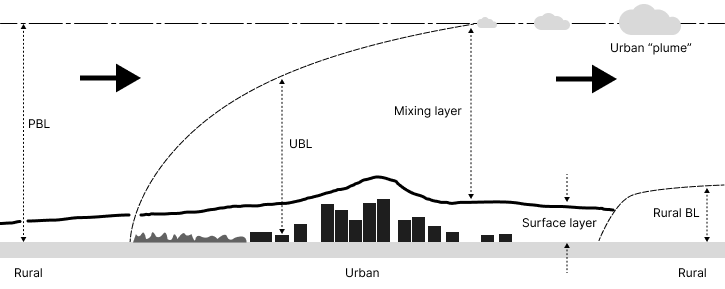
\includegraphics[width=\textwidth]{images/Mesoscale Boundary Layer.png}
    \caption{Mesoscale view of the urban climate, redrawn from~\cite{oke2006guideline}}
    \label{fig:mesoscale boundary layer}
\end{figure}

The mesoscale, as depicted in Fig~\ref{fig:mesoscale boundary layer}, spans the whole urban environment of a city, typically tens of kilometres. There are several boundary layers, that comprise different scales. The planetary boundary layer (PBL)~\cite{wyngaard1985structure} is the lowest layer of the Earth's atmosphere and spans from the surface to a height of several hundred meters up to several kilometres. It is characterised by the turbulent mixing of air, forming wind currents, that are mayorly influenced by the underlying surface.

\begin{figure}[h]
    \centering
    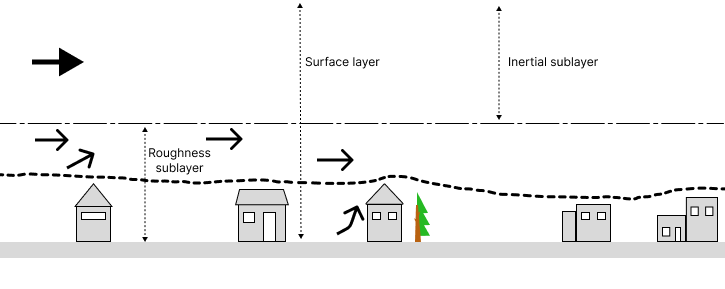
\includegraphics[width=\textwidth]{images/Localscale Boundary Layer.png}
    \caption{Localscale view of the urban climate, redrawn from~\cite{oke2006guideline}, (Todo finish)}
    \label{fig:localscale boundary layer}
\end{figure}

The local scale is situated closer to the surface and contains landscape features such as topography but does not yet include microscale effects. At this layer, the underlying microclimatic effects in form of fluxes mix to form a more average and representative view of the source area, typically at the scale of one to several kilometres. This layer is monitored by weather stations that are located at/or slightly above the canopy height.

\begin{figure}[h]
    \centering
    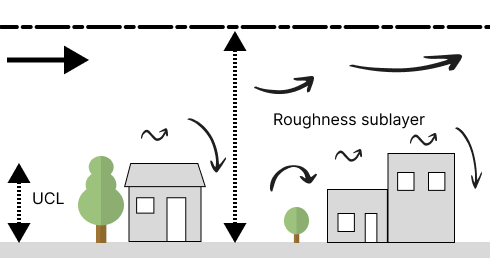
\includegraphics[width=\textwidth]{images/microscale boundary layer.png}
    \caption{Microscale view of the urban climate, redrawn from~\cite{oke2006guideline}, (Todo)}
    \label{fig:microscale boundary layer}
\end{figure}

The microscale usually ranges from a neighbourhood scale to individual street canyons or even microclimates created by individual buildings. It is mayorly influenced by the overall energy balance, which is influenced by cloud coverage, solar radiation and more. Single weather stations are not enough to capture the complex microscale~\cite{oke2004siting}, therefore a dense network of sensors closer to the ground is needed to capture the microscale. Additionally, the microclimate is influenced by surface temperature (LST), however the correlation between air and surface temperature varies greatly based on other surrounding influences such as wind velocity or humidity~\cite{stoll1992surface}, especially in cases of extreme temperatures~\cite{good2016situ}. The closer the air temperature is measured to the surface, the more local the measurement, therefore air temperature of the canopy is usually measured at 2m height, so the different energy fluxes have enough time to mix and form a more representative average for a bigger area.\\
Vertically, UHIs can be divided based on these boundary layers into three mayor types~\cite{oke1976distinction, oke2017urban}, namely Boundary Layer Heat Island (BUHI), Canopy Urban Heat Island (CUHI) and Surface Urban Heat Islands (SUHI), corresponding to the boundary layer they can be measured in. Another differentiating factor is the time of day at which UHIs get detected. For example, Steward~\cite{stewart2011systematic} in his review focussed on night-time UHIs, whereas Peng et al.~\cite{peng2012surface} focussed on both day and night-time UHIs.

\subsection{Surface Urban Heat Island (SUHI)}

The land surface temperature (LST) is measured directly at the surface of an object and is the main indicator of the surface urban heat island (SUHI), which can be found in many cities around the globe~\cite{peng2012surface}. Surface temperature, in contrast to air temperature, is measured via remote sensing technologies via satellites. Well-known satellites include MODIS~\cite{didan2021modis} (NASA), Sentinel 3 (ESA), Meteosat (EUMETSAT), Landsat, and more. The different satellite types carry different types of instruments and sensors, that are able to take various measurements. The used sensor has a mayor influence on the quality of data, e.g.\ resolution via pixel size, robustness against atmospheric influences, ability to handle clouds and more. In Section~\ref{sec:feature_engineering} we discuss other features next to LST that are available via satellite data.\\
Through the use of satellites, the spatial coverage is great, but raster sizes for older satellites such as MODIS usually range from one to several kilometres, therefore the spatial resolution is not as high. For newer satellites such as Sentinel 2 and Landsat, pixel sizes are improved significantly from 10m to 50m, however complementay data such as derived vegetation indexes are usually not available as precomputed values, adding additional work to the data retrievel process, as later discussed in Section~\ref{subsec: remote sensing}.
Additionally, weather satellites usually orbit earth to cover wide areas and are not geostionary, therefore only taking measurements a maximum of 1 to 2 times a day, up to every 16 days or even only once a month, depending on the orbit. As a result, the temporal resolution is quite low and especially in the case of UHI detection, this could mean that the satellite misses the peak of the UHI for a given day or even misses the UHI completely. Another downside is the general inability to take LST measurements through clouds, therefore even if the satellite passes over during a UHI, if there are clouds, the UHI cannot be measured. To alleviate the problem there are new methods such as estimating LST based on emited radiation from clouds~\cite{zhang2015estimation}, however they also have their limitations. Lastly, LST and air temperature are not the same and can vary greatly, especially in extreme heat events~\cite{good2016situ}.\\
To conclude, SUHI analysis can be a good indicator that there is a UHI phenomenon present in a city and can generally direct further research, however it lacks the temporal resolution to be used for real-time UHI detection and is not able to capture microscale effects of the UHI~\cite{voogt2003thermal, voelkel2017towards}.

\subsection{Canopy Urban Heat Island (CUHI)}

The canopy UHI is measured in the canopy boundary layer several meters above ground slightly below or on the average roof layer of the surrounding buildings, as seen in fig.~\ref{fig:microscale boundary layer}. The primary measurement in the canopy is air temperature, which is used to measure the urban heat island intensity (UHII)~\cite{oke1973city}, the most commonly used way of describing the heat island maginitude~\cite{kim2021urban}.\\
Since the beginning of modern climatology, mayor progress has been made in this research field, but methodologies and scientific rigor in CUHI research still seems to be lacking, as discussed by Stewart in 2011~\cite{stewart2011systematic}. Stewart found, that over 54\% of CUHI research was lacking proper methodologies or had other shortcommings such as a lack of site desciptions, where sensors were placed, or the disregard of non-urban factors such as local weather phenomena. In response, progress has been made in recent years by improving methodologies and ensuring correct measurements of climate-related data and study design and execution through various guidelines~\cite{oke2006guideline}, especially in urban settings, that require special care due to the huge amount of possible influences on local recording sites.\\
Additionally, the UHII is highly related to other climatic factors such as wind, cloud cover, and precipitation and is tightly linked to the selection of the recording site~\cite{fenner2019contrasting}, therefore such factors need to be taken into account when measuring the UHII.\\
Compared to LST, TA is measured in situ via weather station networks or other types of sensor networks. Provider for PWS and temperatur sensor networks are further discussed in Section~\ref{sec: private weather station network providers}.

\subsubsection{Shared UHI Challenges}

Some shared challenges for all types of UHI include: 1. Define what \textit{urban} means in the context of UHIs~\cite{stewart2009newly}. The term urban is widely used to identify areas that are more densly populated than the surrounding rural areas. Having this distinction between urban and rural~\cite{lowry1977empirical} helped researchers to better define the UHI magnitude, but this simple distinction also lead to problems~\cite{stewart2011systematic}. The problem lies in the fact that there is no clear border between urban and rural areas, but a fluent transition. Especially for larger metropolitan areas, like Tokyo, the urban area could span 10s to 100s of kilometres, making the collection of reference rural temperatures hard. The reference rural temperature has a direct influence on the UHI magnitude, which is `the most widely recognized indicator of city climate modification in the encironmental sciences'~\cite{stewart2009newly}. As a solution, different classification into local climate zones were proposed~\cite{stewart2012local, stewart2009newly}, that classify areas based on surface roughness, building densities, building heights etc. 2. Measuring the influence of other local urban or meteorologicalphenomena on the temperatures collected. The urban climate is extremly complex, due to many different influences, such as antropological energy, heat dissapated from ACs, vehicles, and more. Additionally, the urban climate is also influenced by surrounding regional/meso-scale climate phenomena such as storms, valleys, mountains, large waterbodies, costlines and more. In Section~\ref{sec:feature_engineering}, we talk about potential features to capture the local urban climate.

\section{Smart Cities}

Smart Cities offer many new possibilities, enabling new ways of communication and sensing applications. In order to find out, how a Smart Cities are structured and how applications could take advantage of data provided by a Smart City, we take a look at its general architecture.
The most generalised architecture of a smart city consists of four layer, the sensing layer, transmission layer, data management, and application layer~\cite{silva2018towards}. In this work, we focus on the sensing layer, dealing with topics such as correct sensor placement and underlying sensor footprints, and the application layer, which accesses available data via data management services to provide additional services to the city and its citizens. For the data transmission and data management layers, there already exist different technologies and service offerings, that aim at solving the underlying problems, e.g.\ network bandwidth, network availability, sensor discoverability, handling the massive amounts of data that is already or will be collected in the future, and many more. For the communication and discovery of sensor nodes, one solution could be SkipNet~\cite{harvey2002skipnet}, an overlay network focused on discoverability while also protecting privacy, with which the data transportation layer could be desinged as a peer-to-peer (P2P) network. Other research focuses on the data accessability and discoverability, by making data accessible for everyone, not only for economic partners in a closed-off system. Examples would be the Smart Networks For Urban Citizen Participation (SANE) initiative~\cite{bornholdt2019sane}, which could provide crowd-sourced distributed air temperature sensing with a framework to make sensors searchable and subscribable, allowing real-time applications by consuming sensor data streams. Figure~\ref{fig:system-architecture-overview} shows how an architecture with SANE could look like.\\
In connection to this work, ML-based interpolation, for example for air temperature, could be used to augment Smart City applications by supplying data for sensor locations while a sensor is offline, or by turning discrete sensor readings into a temperature map that could be used by researchers for further heat related analysis or by decision makers to inform and visualise heat stress in a city.\\

\begin{figure}[h]
    \centering
    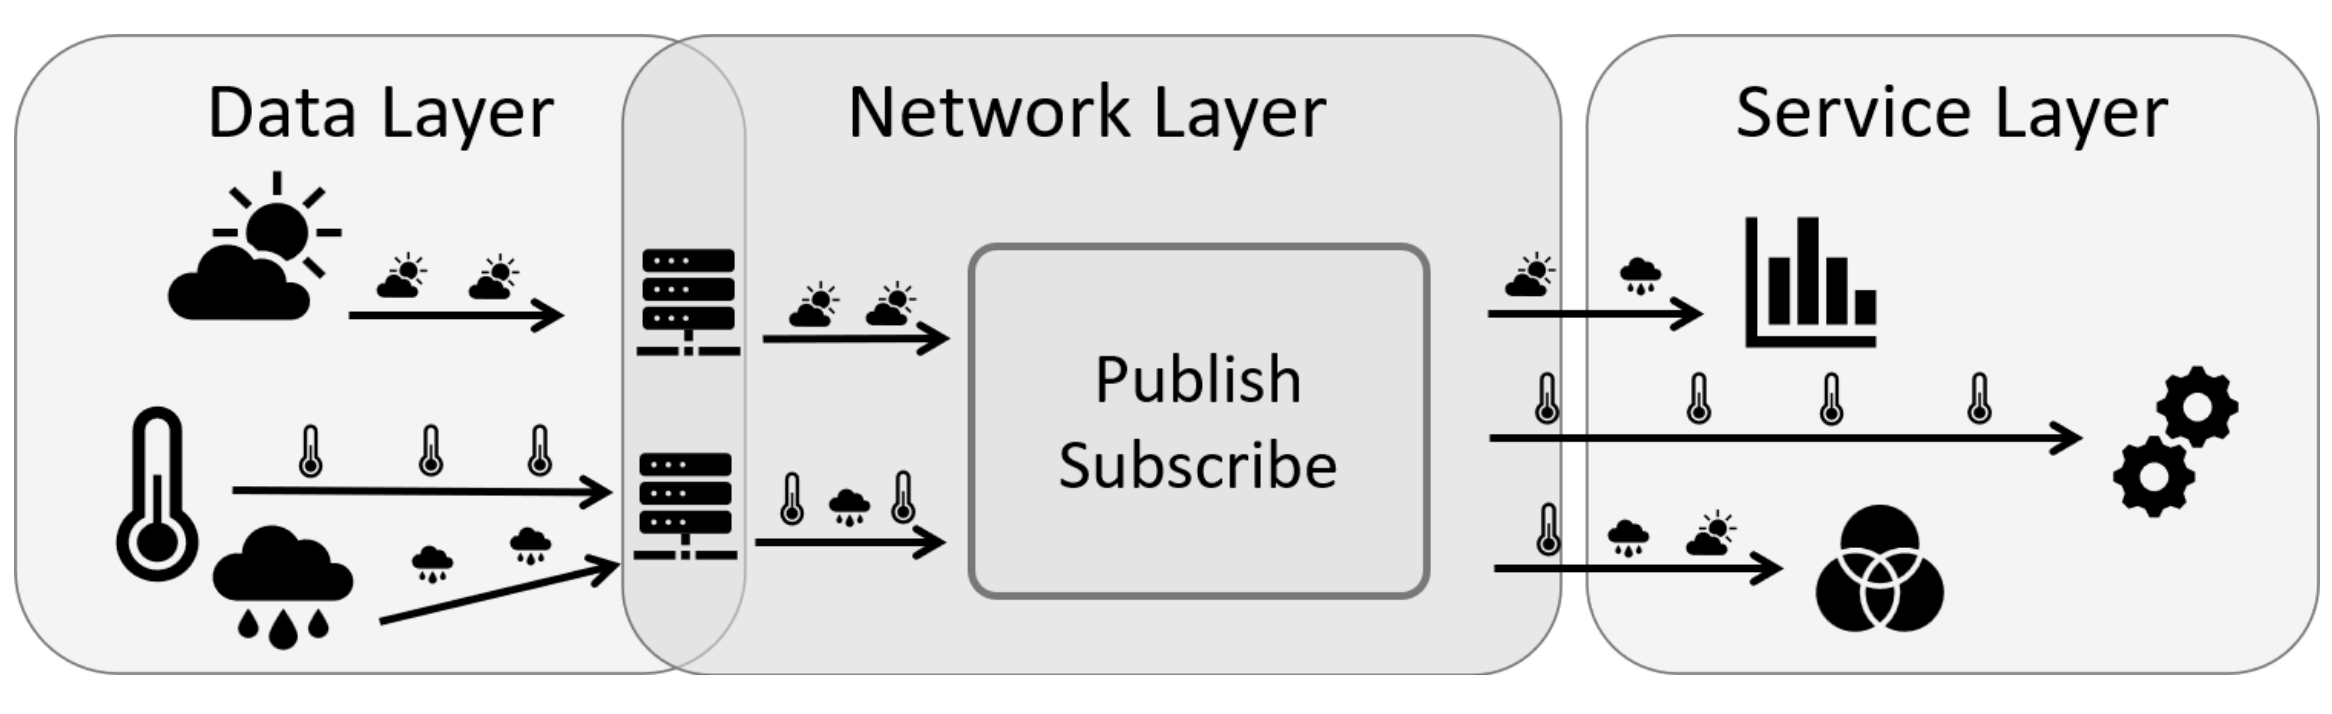
\includegraphics[width=\textwidth]{images/expose-system-architecture.png}
    \caption{In the data layer (left), a wide variety of environmental data is collected with the help of multiple sensors. These are connected to their citizen-owned local base stations, which manage access rights and forward collected data to subscribed services (right) via the decentralized publish-subscribe in the network layer (centre).}
    \label{fig:system-architecture-overview}
\end{figure}

\subsection{Sensing Layer}

The goal for the sensing layer is to monitor the surrounding environment and capture key data for further analysis and decision making. It consists of many different types of physical and virtual sensors. The first group of sensors are the physical sensors, which are placed directly inside the environment. Wireless sensor networks (WSN)~\cite{dargie2010fundamentals} have seen a lot of attention for many different applications such as `military sensing, physical security, air traffic control, traffic surveillance, video surveillance, industrial and manufacturing automation, distributed robotics, environment monitoring, and building and structures monitoring'~\cite{chong2003sensor}. The challenges for WSNs primarily depend among other things on the deployment. An ad-hoc WSN has energy and bandwidth contraints due to the usage of batteries as power sources.
In contrast, sensors that are permanetly installed, either stationary or on a moving target, and connected to a constant power source don't have this constraints. This approach could be used for smart cities to reduce waste and guarantee representative measurements via correct sensor placement. In the case of stationary sensor networks though, the initial deployment and following maintenance cost can be substantial, as seen by the Birgmingham Testbed~\cite{chapman2015birmingham}. If the cost is however distributed across many by following a crowd-sourcing approach, e.g.\ crowd-sensing via PWS, larger networks could be maintained, but there are also new challenges introduced by running a sensor networks by non-professionals~\cite{meier2017crowdsourcing}.\\
In recent years, low-cost sensors (LCS) in combination with sensor networks have enabled fine-granular real-time monitoring of urban environments~\cite{grimmond2006progress, rundel2009environmental}, although the quality of individual low-cost sensors can be questionable~\cite{castell2017can}. Especially PWS data has been used to augment weather data from traditional weather monitoring networks from offical weather services~\cite{hahn2022observations}. In general, LCSs can improve data availibility and support analysis, but do not substitute well-calibrated reference instrumentation~\cite{lewis2018low}.

\subsubsection{Stationary Sensors}

There are many different types of environmental features that can be measured directly inside an urban area. The types of measurements that can be observed are among others: air temperature, humidity, atmospheric pressure, reactive gaseous air pollutant (CO, NOx, O$_3$, SO$_2$), particulate matter (PM), greenhouse gases (CO$_2$, CH$_4$), percipitation, solar radiation, wind speed and direction, anthropogenic heat, noise, sky-view factor, heat fluxes and many more.
Correlations between these features can vary greatly based on surrounding factors. In order to better understand these correlations, many empirical studies have studied the influence of meteological factors on features such as PM~\cite{tai2010correlations}. Additionally, many fields of statistics have specialised on topics such as statistics in climatology~\cite{von2002statistical}, geostatistics~\cite{trangmar1986application} and more.\\
All sensor readings that are taken by physical sensors are singular data points. Additionally to the type of measurement taken and the actual value observed, physical sensor readings include the physical location of the sensor, e.g.\ latitude, longitude and sometimes altitude, the type of sensor used to take the measurement, and sampling rates. For air temperature, the sampling rate could be an average temperature measured over five minutes, whereas percipitation might be measured by collecting rain for certain periods of time and then measuring the amount of rain collected. The sensor type is important, as different types of sensors can produce different qualities of measurements, e.g.\ LCS have lower accuracy compared to callibrated reference-grade high cost sensors and might have lower response rates, and perform better or worse based on the meteological conditions, e.g.\ worse performance at low temperatures, high humidity etc. Due to the placement directly inside the environment, (near) real-time observation and high temporal resolution are generelly possible, but might be influenced by factors such as network availability. The spatial resolution highly depends on the number of sensors deployed and the correct placement of the sensors. The correct placement has a direct influence on the footprint of the sensor~\cite{leclerc2014footprints} and the representativness of the measurement taken for the underlying and surrounding area~\cite{oke2006guideline}.\\
One downside of the placement directly in the environment the sensors are observing, is the exposure to environmental influences such as heat, humidity, or pollution, that can decrease the lifetime of a sensor and may require more frequent maintenance or replacement. On example could be that due to pollution in the air, a rain gauge might be cleaned/replaced more often as over time dirt builds up very quickly.

\subsubsection{Mobile Sensors}

Next to stationary sensors such as a PWS, mobile sensors are not bound to one place, but have the ability to move through the environment they are placed in. This increases the spatial coverage at the cost of temporal resolution, as a sensor is not always in the same place. In the context of urban air temperature sensing, LCS could be mounted to moving vehicles such as busses, cars, e-bikes and scooters, and more. This could help improve the spatial coverage of a sensor network. In combination with ML-based interpolation, such moving sensors could be used to create virtual sensors for specific locations, where a ML model learns the relationship between surounding sensors so that air temperature could be interpolated for times when a moving sensor is currently not a the specific location. In their study, Yang et al.~\cite{yang2019designing} found that randomly mobile sensor networks outperformed completely stationary sensor networks for measuring monthly mean temperatures, however they had higher errors of up to 5°C when measuring daily maximum temperatures. They suggest that hybrid systems with both stationary and moving sensors are more robust in measuring short extreme events such as heat waves.\\
Next to mobile sensor networks, offical weather services such as the DWD also do temperature profile measurements~\footnote{\url{https://www.dwd.de/DE/service/lexikon/Functions/glossar.html?lv2=101996&lv3=102106}, \textit{last accessed: 23.08.2023}}, where sensors are mounted to a car to capture air temperature, humidity, wind speed and direction, as well as possibly atmospheric pressure. This data can be used to support research into local climates. Especially interesting for these profile drives are `summer cloud-free and light-windy high-pressure weather conditions, as then temperature differences between the city and the surrounding area become particularly pronounced and temperature-equalising cold air flows reach their greatest intensity.'~\footnote{\url{https://www.dwd.de/DE/forschung/klima\_umwelt/klimawirk/stadtpl/projekt\_warmeinseln/projekt\_waermeinseln\_node.html}, \textit{last accessed: 23.08.2023}}.

\subsection{Application Layer}

The application layer contains services which utilize data provided by the data management layer to provide services for the city and its citizens. As part of this layer, services could be build that aggregate data streams coming from the data management layer and use ML to improve the data quality by detecting outliers, reducing bias, interpolating missing data etc. The improved data could then be published and other services that would otherwiese rely on the raw data streams and potentially need to implement their own outlier detection or interpolation of missing data techniques, instead simply subscribe to the externally managed service. This could lower the barrier to entry for developers with less available resources, financially or domain-knowledge wise, and generelly allow developers/service providers to allocate their resources to other areas like user experience (UX) and usability compared to the maintenance of complex ML-based services.\\
In the context of this work, we focus on air temperature interpolation and have the motivating factor of UHI detection. In this context, there could be a UHI detection service that ingests real-time data streams from the data management layer and notify citizens if an UHI is detected in or predicted for a particular urban area. As the main challenge for UHI detection lies, next to the definition of urban and rural reference areas, on the gathering of a comprehensive temperature map that allows for UHI detection algorithms to work, in this work we also evaluate areal interpolation of air temperature. Such areal interpolation techniques could then be used to create a temperature map service that enables the detection of CUHIs and could also be used as a foundation for other services in a smart city, like plant watering systems, smart healthcare and more. Examples for (crowd-sourced) temperature maps are later shown in Section~\ref{sec: private weather station network providers}, as many PWS providers also operate a temperature map as well. The problem here is that every provider has its own temperature map with custom ways of storing and accessing the data, making it difficult and time consuming to work with different providers.

\section{Interpolation}

Interpolation is in essence to determine unknonwn data points based on a set of given data points~\cite{steffensen1927interpolation}. In this work, we focus on spatial interpolation which is the interpolation problem applied to spatial data given either as discrete data points or subareas, to determine a complete area. First, we categorize and introduce different spatial interpolation methods to get an understanding about what methods exist and which method is preferred in which application area based on the literature review by \textit{Lam} from 1983~\cite{lam1983spatial}, and augment certain areas with the current state of research. In recent years, many more specialised interpolation methods have been developed for really specifc use cases, as interpolation is not only about randomly selecting values, but estimating data points based on assumptions about the relationship with the existing data points and the area to interpolate. Depending on the exact use-case, these assumptions could be about the distribution of the data, or as a specific example in the case of interpolating liquids, having constraints such as volume-preservance.\\
Generally, spatial interpolation methods can be categorised by many different factors. Lam differenciated between point interpolation, which is either exact or approximate, and areal interpolation, which is either non-volume-preserving and the same as point-based interpolation, or volume-preserving. As in-situi sensor readings are singular data points at discrete locations, we focus on point interpolation, but note here that such data points could also be mapped into a partial grid first to then use areal interpolation methods.
Point interpolation methods can either be exact, meaning that the original data points are preserved 1 to 1 in the interpolated area, or approximated, e.g.\ they are fitted to a function that does not necessarily pass through all original data points. The important methods are as follows:

\begin{itemize}
    \item Exact

    \begin{itemize}
        \item Weighting
        \item Kriging
        \item Splines
        \item Interpolating Polynomials
        \item Finite Difference
    \end{itemize}

    \item Approximate

    \begin{itemize}
        \item Power Series Trend
        \item Fourier Series
        \item Least-squares Fitting with Splines
        \item Distance-weighted Least-squares
    \end{itemize}
\end{itemize}

\subsection{Exact Point Interpolation}

Exact point interpolation methods have the benefit that the original data points are preserved. Fitting the original data points to a polynomial is the simplest form of interpolation, however it has the mayor drawback that there are no additional constraints for points that are not part of the original data set, potentially resulting in highly unreasonable estimations.\\
The main idea of weighting methods is the idea to assign more weight to data points that are closer than points that are further away. Due to it's simplicity and fast computation, inverse-distance weighting (IDW)~\cite{willmott1985small} is a popular and commonly used interpolation method. The main downside with IWD is that it is a smoothing technique, therefore it is not able to capture local maximas and minimas, which could be critical for UHI detection. Splines~\cite{mitavs1988general}, another exact smoothing technique, is a mathematical method that fits either a smooth curve or surface to a set of given points. It offers several advantages such as smoothness and retention of small-scale features, however this method can be computationally expensive and might not be best suited for highly irregular data points, e.g.\ big differences between data points located very close to each other. Finite Difference is a method to caluclate a surface based on a set of differential equations, which can calculate a smooth surface from the given points, however at the cost of higher computational cost to solve the differential equations itteratively.\\
Kriging, a geostatistical interpolation method, originally developed by Krige~\cite{krige1976review} as a moving averaging technique to reduce global biases, has developed into one of the most prominent spatial interpolation methods and has seen many contributions and improvements since the introduction of Ordinary Kriging (OK) and Universal Kriging~\cite{li2014spatial}.

\subsubsection{Kriging}

Due to its popularity, we discuss Kriging methods in more detail. Kriging methods use a covariance function to model the spatial correlation between data points~\cite{wackernagel2003multivariate}. The covariance function is a measure of the similarity between two data points, which is used to calculate the weight of the data point in the interpolation process. There are different types of Krigin methods available, each suited for different use cases, as offered by ArcGIS~\footnote{\url{https://desktop.arcgis.com/en/arcmap/latest/extensions/geostatistical-analyst/what-are-the-different-kriging-models-.htm}, \textit{last accessed: 24.08.2023}} including:

\begin{enumerate}
    \item Simple Krigin: the simplest form of Krigin, that assumes that the mean of the measured values is known and constant
    \item Ordinary Krigin: same as Simple Krigin, but the mean is an unknown constant
    \item Universal Krigin: instead of assuming a constant mean, the mean is modeled as a deterministic function
    \item Indicator Krigin: same as Ordinary Krigin, but for categorical data
    \item Propability Krigin: same as Indicator Krigin, but assumes two types of random errors that can are each auto-correlated and cross-correlated to each other
    \item Disjunctive Krigin: same as Ordinary Krigin, but tries to improve the prediction quality by using an unknown constant and approximating an arbitrary function. It requires the bivariate normality assumption and is difficult to verify and solutions might be mathematically and computationally complicated
    \item Cokrigin: offers methods for the previous Krigin methods, but uses information on several variable types. This could improve the prediction quality, but might increase the variance of the prediction, as more much more estimation is required
\end{enumerate}

In the context of geostatistical analysis, there are different types of Krigin methods available that combine the aforementioned methods with other techniques, such as regression analysis. The following list is the geostaticial methods offered by ArcGIS Pro as part of the Geostatistical Analyst toolbox~\footnote{\url{https://pro.arcgis.com/en/pro-app/latest/tool-reference/geostatistical-analyst/an-overview-of-the-geostatistical-analyst-toolbox.htm}, \textit{last accessed: 24.08.2023}}:

\begin{enumerate}
    \item Empirical Bayesian Krigin (EBK)
    \item Empircal Bayesian Krigin 3D (EBK3D)
    \item EBK Regression Prediction (EBKRP): Empirical Bayesian Kriging with regression prediction
    \item Global Polynominal Interpolation
    \item Kernel Interpolation with Barriers
    \item Moving Window Krigin
    \item Radial Basis Function
\end{enumerate}

ArcGIS Pro is a paid service, therefore we only take a look at openly available implementation, more precisely the Kriging implementation from the Python library \textit{PyKrige}~\cite{benjamin_murphy_2022_7008206}, which are the following:

\begin{itemize}
    \item Ordinary Kriging
    \item Universal Kriging
    \item Regression Kriging
\end{itemize}


	% Machine Learning based Interpolation
	\chapter{Machine Learning-based Interpolation}
\label{chap:Machine Learning based Interpolation}
% 10 pages?

% Intro with small motivation why ML is used
In recent times, the area of machine learning has seen big advancements in terms of model size and complexity. Especially in the area of generative AI, transformer-based neural networks have revolutionised text and image generation. Models such as OpenAI's \textit{ChatGPT}~\cite{openai2023gpt4} or Google's \textit{LaMDA}~\cite{thoppilan2022lamda} have generated significant hype for the possiblity of use of AI\@. Additionally, statements like the universal approximation theorem, which states that a feed-forward network with a single hidden layer containing a finite number of neurons can approximate any continous function~\cite{hornik1989multilayer}, emphasize the potential power of ML models.
As a result, the question arises what benefits AI can bring to other areas of application, such as interpolation. In this chapter, we will discuss the usage of ML in the context of data enrichment via interpolation, more precisely in the context of smart cities and air temperature interpolation, and outline possible advantages and disadvantages compared to traditional (geo-) statistical methods.\\
% TODO: emphasize the usefulness for handling dynamic data, such as moving sensors
% ML in the context of the goal of this work
Because ML is such a powerfull tool, in this chapter we will discuss how ML can be used for contextual data enrichment via interpolation, specifically in the context of smart cities and air temperature sensing applications. More specifically, as meteorological research and analysis activities are usually in need of gridded or continuous data~\cite{sekulic2020spatio}, the goal of this chapter is to design a ML model that is capable of turning these single data-points into a gridded data layer of air temperature where each cell has a specific air temperature value. Furthermore, traditional (geo-) statistical approaches have certain limitations such as potentially lower flexibility. In the context of temperature interpolation, another important question to discuss is how moving sensor data can be incoporated into the model in addition to statinary sensors and weather stations.\\ 
In the following, we first take a look at the taxonomy of ML algorithms in order to understand which interpolation tasks ML can solve, before deciding on a number of potential ML models for the task of air temperature interpolation, which will later be implemented and evaluated.

\section{AI vs. Machine Learning vs. Deep Learning}

Before diving deeper into the applications of ML, we need to clarify what is meant by artificial intelligence (AI), machine learning (ML) and deep learning (DL). AI is a broad term that is used to describe the ability to perform tasks, that are usually associated with human intelligence. ML is a subfield of AI, that focuses on the ability of a system to learn from data without being explicitly programmed to do so. Finally, DL is a subfield of ML, that uses artificial neural networks, which imitate the structure of the human brain, to learn from data and perform various tasks.\\
% TODO: graphic?

\section{Taxonomy of Machine Learning Algorithms}

% classification vs regression
% supervised vs unsupervised vs reinforcement learning

Generally speaking, ML algorithms can be categorised based on many different properties~\cite{sarker2021machine}, such as the type of learning, e.g. supervised, unsupervised, semi-supervised or reinforment, or the type of problem they try to solve, e.g. classification, regression or clustering. The most important differenciation for this work is to distinguish algorithms based on the type of problem they try to solve. Because we focus on solving interpolation problems, in this work we will only consider algorithms that can be used to solve regression problems, as interpolation is a form of regression.\\
In regression analysis, the goal is to predict a (continous) target variable $y$ based on a set of input variables $X$ (cite), like it is the case for temperature interpolation. Generally speaking, this problem can be classified as a supervised learning problem, therefore the possible algorithm candiates are as follows:

\begin{itemize}
    \item Linear Regression
    \item KNN Regression
    \item Regression Trees and Random Forests
    \item Tree Boosting
    \item Support Vector Regression
    \item Neural Networks
\end{itemize}

Each model has certain benefits but also comes with drawbacks or special assumptions for the input data to the model. First, we will discuss each model and then compare these assumptions with the data coming from the data-layer, to identify suitable models for the task of air temperature interpolation. These models will then later be implemented and compared in chapter \ref{chap:Evaluation}.\\
Based on the domain, there already exist proposed best-practices for which algorithms to use for what applications. In the context of smart cities such recommendations for topics such as intelligent transportation systems, smart grids, smart city health care and more can be found in \cite{ullah2020applications}, which unfortunately does not cover interpolation.

% TODO: table with model comparison for quick overview

\subsection{Linear Regression}
\label{subsec: linear regression}

Linear regression~\cite{montgomery2021introduction} is a comparatively simple, yet very popular and widely used model for regression problems. The goal of this model is to predict a continous dependent variable based on a number of independent variables. These independent variables can be either continous or discrete. The model can be expressed as follows:

% TODO: explain equation
\begin{equation}
    y = \beta_0 + \beta_1 x_1 + \beta_2 x_2 + ... + \beta_n x_n + \epsilon
\end{equation}

The relationship between the parameters is assumed to be liniear, while each variable must be independent of each other. Due to this independent assumption, there are special steps needed to make linear regression work for (geo-) spatial data, as these types of variables are usually correlated with each other.

\subsection{Regression Trees and Random Forests}

Decision trees are used for a wide variety of classification problems. Due to the fact that decision trees can vary significantly given similar inputs, e.g have a high variance, random forests were introduced as a counter measure. Random forests combine multiple decision trees and average their predictions in order to reduce the variance.\\ 
When instead of a discrete target variable a continous target variable is predicted, regression trees can be used. The principle behind regression trees is to split the data into continously smaller sub-sets, and asking the correct questions at the right time in order to find the best split. Compared to decision trees which try to minimise the entropy, regression trees try to minimise an error that is compatible with a continous target variable such as mean squared error (MSE). The model can be expressed as follows:

% TODO: explain equation
\begin{equation}
    \hat{y} = \sum_{m=1}^M c_m \mathbb{1}(x \in R_m)
\end{equation}

Regression trees are easy to understand and interpret. Additionally, they do not require any scaling of variables, which is a big advantage compared to other models. However, they are prone to overfitting and are not suitable for extrapolation. Furthermore, they are discontinous at the split points, which is a big disadvantage for interpolation of spatial data. Therefore, regression trees don't seem to be suitable for the task of air temperature interpolation.

\subsection{Tree Boosting}

% TODO

\subsection{Support Vector Machines}

Support Vector Machines (SVM) are typically used in classification problems, however they can be also used for regression problems, called Support Vector Regression (SVR). SVMs transform the input data into a higher dimensional space and try to find a hyperplane that separates the data into two classes. This approach is similar to linear regression, however SVMs are more robust to outliers and can be used for non-linear problems. Depending on the Kernel function used, e.g. Linear, Polynomial, Radial Basis Function (RBF) or Sigmoid, the model can suffer from the same problems as linear regression when dealing with correlated spatial data.
As a result, appropriate counter measures need to be taken, such as using the Mahalanobis distance instead of the Euclidean distance for RBF kernels~\cite{kamada2006support}, which converts correlated features into uncorrelated features.

\subsection{Neural Networks}

Neural networks 

\subsubsection{Deep Neural Networks}

% TODO

\section{Model Assumptions from the Data Layer}

Next to the model, the most important thing for a machine learning algorithm is the data. Even when the model is perfectly suited for the task at hand, if the data is not suitable, e.g. not enough data, wrong quality, wrongly prepared or formatted etc., the model will not be able to perform well. In the following, we take a look at the data coming from the data-layer and discuss important assumptions such as spatial and temporal autocorrelation. These correlations are important to consider, as they could invalidate models as f.e. Linear Regression~\ref{subsec: linear regression} assumes uncorrelated input variables.\\
First of all, the data-layer exposes a variety of single data-points for various features for different locations for current and past points in time.
.Features other than air temperature could further improve the predecition quality, like how~\cite{alonso2020new} suggests that in their study the Normalized Difference Vegetation Index (NDVI) and Modified Normalized Difference Water Index (MNDWI) have a strong impact on their estimation model. Therefore, we discuss how additional features can be included in the model.\\
This model should then be deloyed inside the \textit{service-layer} and act as a building block for further temperature related research and analysis, as air temperature is an important variable for research in agronomy, meteorology, hydrology, ecology and many other fields of application and could be used for UHI detection in the context of smart cities. The general idea and architecture behind the model should not only be applicable for air temperature, but also other types of output features, even tho potentially significant domain knowledge, like in geostatistical analysis and statistics, is required to select and prepare the input features.\\
% TODO: summary of the assumptions for the geolocation data
Generally, there are different types of input features. Firstly, there are discrete measurements that capture the underlying continuous geological process as a specific value at a certain point in time. Examples for this are the measurements from sensors which might be deployed in an urban environment to capture air temperature, humidity and more. Important to note here is the interval, the values are captured. For example, a sensor might capture the air temperature as the average over five minutes, whereas a rain sensor might capture the absolute amount of rain in a specific time interval. Secondly, there are calculated features, which might be derived from the discrete measurements or the location of a measurement. For example, the distance to the closest body of water with a minimum size of $x^2$ meters might be a important information for the air temperature. Lastly, ...\\
% data from gridded data sources (e.g. affiliation to postal code, district...)
In the following chapter, we discuss how different types of correlation between measurements can be taken into account to improve the model and gain additional insights into local (meteological) dynamics.

\subsection{Spatial Autocorrelation}
% How different measurements are spatially related inside a time series

As discussed in chapter \ref{chap:Related Work}, there is a dependency between air temperature and other meteological features and the location of the sensors. The closer a sensor is to another sensor, the more correlated the sensor readings should be.
In geo-statistics, this is called spatial autocorrelation and can be defined traditionally with the Moran's I index~\cite{moran1948interpretation} or the Geary's coefficient~\cite{geary1954contiguity}. 
% TODO: explain autocorrelation and the implications for ML models
% model assumptions: no ML algorithm that expects independence between observations
% feature selection: including all correlated features can lead to overfitting
% spatial feature engineering: add additional features that encode the spatial relationship between sensors
% spatial smoothing:
% spatial aware algorithms: geographically weighted regression (GWR) 

This relationship is however greatly influenced by the type of feature and the location of a sensor. As explained in \cite{oke2006guideline}, the sensor placement in the urban environment is a complex task, as the urban environment is highly dynamic and sensors can be influenced by highly local phenomena, such as air temperarture by heat vents or solar radiation by buildings and surface materials. For this model, we assume that the sensors are placed in a way that the sensor readings are representative for the area they are placed in, even tho in practice this assumption might not hold up, especially for sensors placed by non-experts.\\
Each sensor reading from the data-layer has a location associated with it in the form of longitute, latitude and altitude (if available). This information can be used to calculate the distance between sensors and subsequently the correlation between sensor readings. However, how exactly the distance between two locations is calculated is not trivial. As the earth is a sphere, the distance between two points on the surface is not a straight line. Depending on the application, different distance metrics can be used. For a small area, such as the city of Hamburg, the euclidean distance could be sufficient, as the curvature of the earth for a small distance is negligible. However, for larger areas the geodesic (harvesine) distance might be more appropriate. In this work, we are focussing on a single city including it's surrounding area, therefore the euclidean distance should have a sufficient accuracy while also simplifing the calculation. As the city of Hamburg does not have big differences in elevation, the altitude is not considered in the distance calculation.\\
% grid area -> each data point is in a grid cell. Multiple data points can be in the same grid cell. If this is the case, the readings are averaged. Outliers based on the overall mean temperature are removed. -> this is done in the data layer
The location data can be incorporated into the input data in several ways. The most straight forward way would be to just include the longitude and latitude as input features. Depending on the type of model used, these values might need to be normalised. For example, tree-based models do not require normalisation (cite), as they are not sensitive to the scale of the input features. However, neural networks are very sensitive to the scale of the input features and therefore require normalisation (cite). This approach has the downside, that the distance between sensors is not directly encoded in the input data. If this information is important for the model, it could be included by precalculating the distances between all sensors, however this would increase the complexity of the model especially for large amounts of sensors, as this would result in a quadratic number of input features.\\
The next approach would be to convert the 

- area n x m grid of data points, each grid cell with n x n size (depending on the resulution), 4D space with location as x and y coordinates (euclidean distance -> but only for smaller areas such as city of Hamburg and suroundings), time as z coordinate and feature values as w coordinate.\\

\subsection{Temporal Autocorrelation}
% How different measurements are temporally related inside a time series


\subsection{Temporal Cross Correlation}
% How different time series are related to each other (seasonaility)

% TODO
\subsection{Dealing with Correlation}

Todo: Techniques to turn correlated variables into uncorrelated ones
- principal component analysis (PCA)
- ...

\subsection{Dealing with Uncertainty}
- The model has a lot of uncertainty
- model uncertainty in input data? (depending on sensor type, sensor age, placement...)

- dealing with bias
- dealing with variance
-> problem of over-fitting

\subsubsection{Neural Network Models}
input layer -> hidden layers -> output

The advantages of Multi-layer Perceptron are:
- Capability to learn non-linear models.
- Capability to learn models in real-time (on-line learning) using partial\_fit.

The disadvantages of Multi-layer Perceptron (MLP) include:
- MLP with hidden layers have a non-convex loss function where there exists more than one local minimum. Therefore different random weight initializations can lead to different validation accuracy.
- MLP requires tuning a number of hyperparameters such as the number of hidden neurons, layers, and iterations.
- MLP is sensitive to feature scaling.

- Loss functions/optimzers: Stochastic Gradient Descend, Adam, L-BFGS


- random forest regression
...

\subsection{Evaluation Metrics}
- Mean absolute error, mean absolute relative, mean quared error, r-squared, root mean squared error (RMSE)

\section{ML Model Deployment}
Deployed as a service. Input ingested -> continous data map as output all 5 min or so (could also be smaller depending on use-case -> trade-off between cost and accurancy)

\subsection{ML Model Retraing}
Need to retrain model from time to time, e.g. if the accurracy drops below a certain threshold.


% Implementation details
- dealing with coordinate systems:
    - projected coordinate system (e.g. UTM) instead of long lat alt values (important for interpolation)

\section{Machine Learning in Geostatistics}

Idea/Hyphothesis: ML outperforms traditional geostatistical models (in certain scenarios) as it is able to capture more complex interdependencies between features and isn't necessarily bound to the (mathematical) assumptions of geostatistical models.

On important point to mention, is that different meteological features have different interpolation techniques, as they beve different (physical) properties. For example, temperature is a scalar value, while wind speed and direction are vector values. Relative humidity on the other hand is a relativ value that is bound between 0 and 1. For percipitation it gets even more complex, as rainfall is highly connected to cloud coverage and movements. In the following, we will take a look at commonly used existing interpolation techniques for different meteological features and discuss data preprocessing steps.

- Dealing with sparse data
- Dealing with extreme weather events (e.g. heat waves, blizzards, etc.)
- how can a ML model be trained if no such data exists for a given area? -> transfer learning

\subsection{Temperature Interpolation}
- difference between air and surface temperature

surface temperature -> solar radiation, surface roughness, emissivity, soil moisture, soil temperature, vegetation cover, snow cover, and surface slope

air temperature -> surface temperature

\subsection{Wind Speed and Direction Interpolation}
prob not easily archivable with ML -> depends on high/low pressure areas

\subsection{Relative Humidity Interpolation}
Data preprocessing: scale to [0, 1]
does not seem to work well with kriging, maybe just nearest neighbor approach/linear, or the input values are just not accurate

\subsection{Percipitation Interpolation}



DeepLearning Lecture
- sequence modeling design criteria
    - handle variable-length sequences
    - track long term dependencies
    - maintain information about order
    - share parameters across the sequence

% TODO: quick implementation summary
The model is implemented following advice from~\cite{rey2023geographic}...


	% Data Set Preparation
	\chapter{Preparation of Datasets}
\label{chap:preparations data sets}

Next to the \gls{ml} model selected, the data used to train and evaluate the model has a major influence on its performance. If the data is not representative or information is missing about the underlying process that the model should be fitted to, there can be errors, bias, or an inability to generalize well to new data. In this chapter, we look at potential features for \gls{ta}, at data sources for these features, and discuss the construction process of the datasets used in this work.\\
% Overall dataset availability
In the field of natural language processing and computer vision, there is an abundance of large available datasets which have a big contribution to the advancements in the field, like annotated datasets as provided by Google Research~\footnote{\url{https://research.google/resources/datasets/}, \textit{last accessed: 05.08.2023}}. In comparison in the field of climate research, there are also many datasets, including satellite data, weather station data, and climate model data; however, they are highly distributed or often not openly available. Platforms such as \gls{gee}~\cite{gorelick2017google} try to address this issue; however, the dataset catalogue~\footnote{\url{https://developers.google.com/earth-engine/datasets}, \textit{last accessed: 05.08.2023}} is still limited and does not include datasets offered by local authorities or other research institutions, such as universities.\\
% How does the perfect dataset for \gls{ta} look like?
For the specific use case of temperature interpolation in urban areas, an optimal dataset would contain high spatial and temporal resolution sensor data, e.g., a high sensor density and a low time interval of for example five to ten minutes. Additionally, the sensor placement and sensor quality have a high influence on the accuracy of the sensor readings~\cite{oke2006guideline}, therefore the correct placement and calibration of the sensors needs to be guaranteed. Such requirements are not met by traditional weather station networks as the spatial coverage is too low, as a single weather station is not enough to capture the urban microclimate~\cite{oke2017urban}. The weather station locations of the \gls{dwd} are shown in figure~\ref{fig:dwd sensor locations germany}, which shows that usually at most one weather station is available per city. The weather stations however offer a high temporal resolution in addition to very high-quality sensors, which is why they can be used as reference stations for quality control of other sensors, as discussed in section~\ref{sec:quality control}.\\
A solution to the problem of low spatial coverage is the usage of sensor networks. There are several projects that run dense urban-climate monitoring networks~\cite{muller2013sensors} such as the Helsinki Testbed~\cite{koskinen2011helsinki} or the Birmingham Urban Climate Laboratory~\cite{warren2016birmingham}; however, access to those datasets is limited, for example due to outdated links or the need to request access. Due to the high cost of running such dense sensor networks with high sensor and maintenance costs, professionally run sensor networks are rare and are often only run for a limited period until project funds run out.\\
As an alternative, sensor networks can also be crowdsourced and run by citizens, distributing the cost of individual sensors as well as maintenance costs among many. Especially with advances in sensor technologies, lost cost and compact sensors are more affordable than ever while still providing good data quality~\cite{grimmond2006progress, rundel2009environmental}. In the context of meteorological data, such sensor networks are often referred to as \gls{pws}~\cite{meier2017crowdsourcing} or \gls{pws}~\cite{hahn2022observations} networks. In this work, we use the term \gls{pws}.\\
The main downside of this approach is the lack of quality control and meta data, as the sensors are usually placed by non-professionals in suboptimal locations, e.g., in direct sunlight or too close to walls, leading to incorrect readings or bias in the data. A lack in meta data can also lead to issues, if for example exact positions of the sensors are not known and information about the height of the sensor above ground is missing. However, other concerns such as data privacy also need to be accounted for, as such weather stations are often placed on private property.\\
In this work, data from \gls{pws} networks is used to create datasets for the training and evaluation of \gls{ml} models for \gls{ta} interpolation. In the following sections, we look at available \gls{pws} providers and their data and potential features for \gls{ta} interpolation, discuss additional pre-processing steps such as quality control or sensor height correction, and finally discuss the construction of the datasets used in this work.

\section{Private Weather Station Network Providers}
\label{sec: private weather station network providers}

\gls{pws} providers offer a platform for users to upload their sensor data and either sell weather stations and sensors themselves (e.g., Netatmo) or provide guides to allow users to connect their own sensors to the platform (e.g., Sensor.Community). Netatmo data in particular has been used in several studies~\cite{meier2017crowdsourcing, hahn2022observations, venter2020hyperlocal, zumwald2021mapping} and has seen complementary studies for example discussing \gls{qc}\\
processes~\cite{fenner2021crowdqc+}, later seen in Section~\ref{sec:quality control}. There are also other \gls{pws} network providers such as Sensor.Community or \gls{wow} that have been used in several studies~\cite{ho2014mapping}. To find out which provider best fits our needs in this work, the following section compares the different providers and their data.

\subsection{Sensor.Community}

Sensor Community~\footnote{\url{https://sensor.community/en/}, \textit{last accessed: 05.08.2023}} is a contributors driven global sensor community that creates Open Environmental Data and has an archive~\footnote{\url{https://archive.sensor.community/}, \textit{last accessed: 05.08.2023}} of their historical sensor data world-wide. There are no quality measures recorded for each sensor, but as crowd-sourced sensor data tends to have a lower quality than professionally setup sensors, e.g., sensor placement by non-professionals, we need to explore how the data quality looks like.
In Figure~\ref{fig:temperature_sensor_community_map}, where we see the greater Hamburg area with a currently reported temperature of 25°C by the \gls{dwd} Fuhlsbüttel station, there are multiple sensors that report a temperature of 30°C and above, which could be either due to the sensor being placed in direct sunlight or due to the sensor being faulty. An outlier near Pinneberg is shown in Figure~\ref{fig:temperature_sensor_community_outlier}, where one sensor reports 25°C, as currently expected, and one sensor reporting 50°C, which is clearly an outlier. This data quality issue needs to be addressed in the data pre-processing step and can result in a significant reduction of available data. This was also an issue discussed in~\cite{meier2017crowdsourcing}, as ``erroneous metadata, failure of data collection, and unsuitable exposure of sensors lead to a reduction of data availability by 53 \%``.
From a meta-data perspective, there is no information on the sensor height above ground as well as no quality measures for each sensor, or information on the sensor location accuracy.

\begin{figure}[ht]
    \centering
    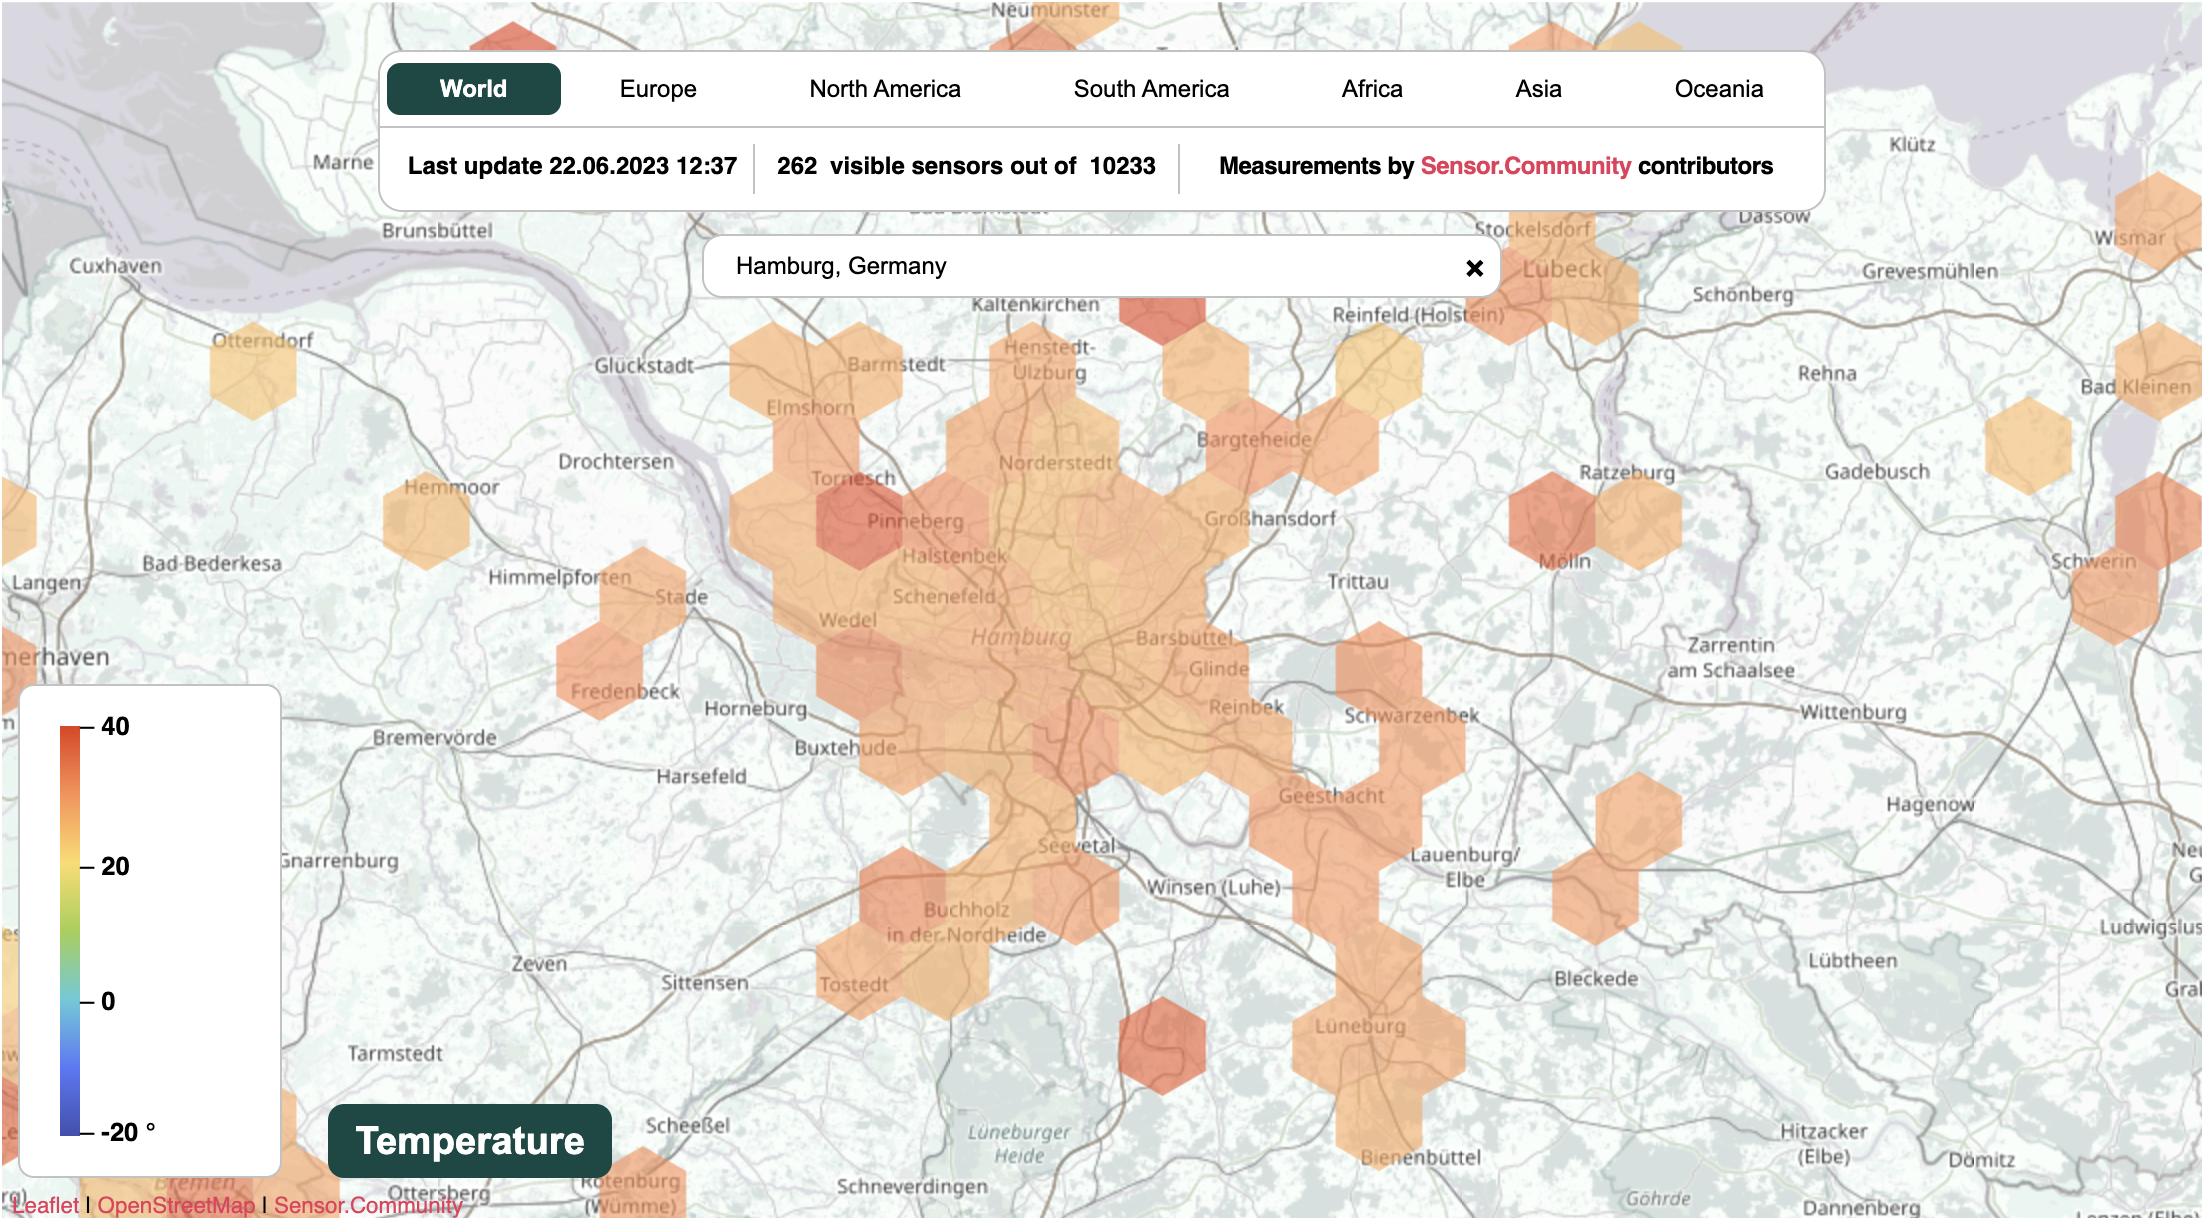
\includegraphics[width=1\textwidth]{images/sensor_community_temperature_map.png}
    \caption{Temperature map from Sensor Community for Hamburg, Germany, on 22.06.2023 12:51h with the \gls{dwd} reference at 25°C}
    \label{fig:temperature_sensor_community_map}

    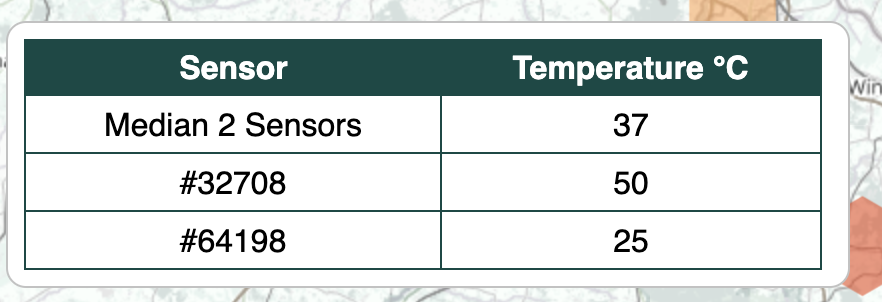
\includegraphics[width=0.8\textwidth]{images/sensor_community_outliers.png}
    \caption{Temperature outlier from Sensor Community for Hamburg, Germany, on 22.06.2023 12:51h with the \gls{dwd} reference at 25°C}
    \label{fig:temperature_sensor_community_outlier}
\end{figure}

Overall, there are around 11.738 active sensors~\footnote{as of 24.06.2023}. Of these sensors, many are located in Germany, as seen in Appendix~\ref{sensor_community_sensors_by_countries}, and almost half of them are of type BME 280, which is a lost-cost Bosch sensor which can measure temperature, pressure, and humidity. The sensor locations as of May 2023 are shown in~\ref{fig:sensor community sensor locations germany}. DHT22 sensors can measure temperature and humidity, BMP280 and BMP180 sensors can measure temperature and pressure, and BME280 sensors can measure temperature, pressure, and humidity.\\

\begin{figure}[ht]
    \centering
    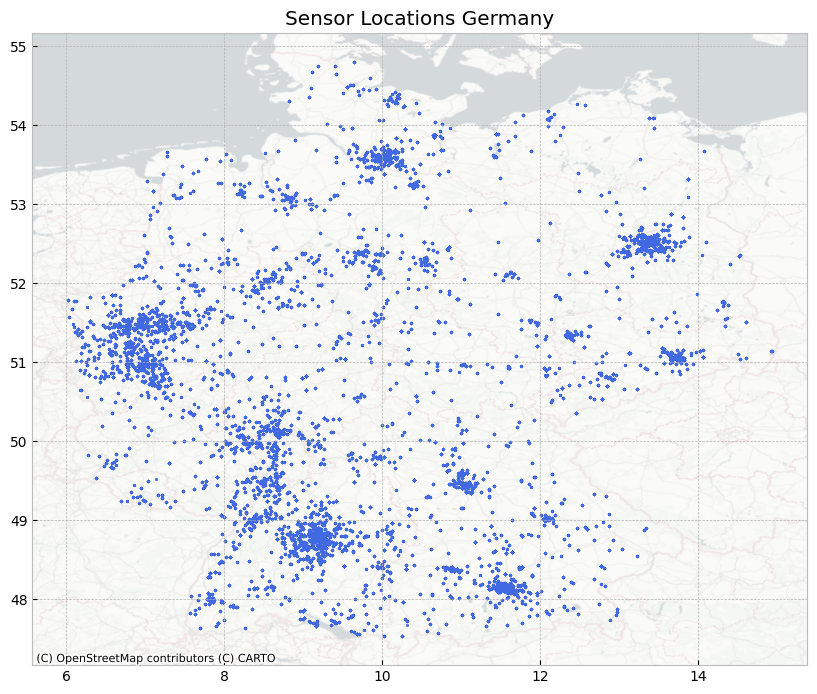
\includegraphics[width=1\textwidth]{images/sc_sensor_locations_germany.png}
    \caption{Sensor locations of Sensor Community in Germany, as of 01.05.2023, of sensor type DHT22 (2590 sensors), BME280 (1558 sensors), BMP280 (100 sensors), BMP180 (72 sensors)}
    \label{fig:sensor community sensor locations germany}
\end{figure}

\subsection{Netatmo}

Netatmo~\footnote{\url{https://www.netatmo.com/en-eu}} is a French company that sells smart-home devices including outdoor weather stations, indoor sensors for air quality, as well as other products such as smart cameras. They host a weather map~\footnote{\url{https://weathermap.netatmo.com/}, \textit{last accessed: 06.08.2023}} where customers can share their outdoor weather station data. They provide an API to access current weather station data as well historic data from individual outdoor sensors and modules.
They provide their historical and current weather data for commercial partners or partners in the research and education sector. They are part of the \gls{eumetnet} project~\footnote{\url{https://www.eumetnet.eu/}, \textit{last accessed: 06.08.2023}} which is a network of 31 European meteorological and hydrological services. The project aims to facilitate the exchange of weather data and to improve the quality of weather forecasts, especially in the context of \gls{pws}~\cite{hahn2022observations}. There are currently no openly historical datasets available from Netatmo data, only private datasets~\footnote{\url{https://catalogue.ceda.ac.uk/uuid/e8793d74a651426692faa100e3b2acd3}, \textit{last accessed: 06.08.2023}} that are only available for partners such as \gls{eumetnet} members. They offer an educational program~\footnote{\url{https://www.netatmo.com/en-eu/weather-with-netatmo}, \textit{last accessed: 01.09.2023}} to access temporally and spatially limited amounts of data that is usually only available to commercial partners.

% precisions
% Please add the following required packages to your document preamble:
% \usepackage{booktabs}
\begin{table}[]
\begin{tabular}{@{}lllll@{}}
\toprule
Measurement    & Unit    & Measurement Range      & Precision  & Recording Frequency              \\ \midrule
Temperature    & °C      & -40°C to 65°C          & 0.3°C   & averaged over 5 min              \\
Humidity       & \% (RH) & 0 to 100\%             & 3\%     & -                                \\
Air Pressure   & mbar    & 260 to 1160 mbar       & 1mbar   & -                                \\
Noise          & dB      & 35 to 120 dB           & -       & -                                \\
Wind Speed     & m/s     & 0 to 45 m/s (160 km/h) & 0.5 m/s & every 6 sec, averaged over 5 min \\
Wind Direction & °       & 0 to 359°              & 5°      & every 6 sec, averaged over 5 min \\
Rainfall       & mm/h    & 0.2 to 150 mm/h        & 1mm/h   & every 5 min (bucket is emptied)  \\ \bottomrule
\end{tabular}
\caption{Netatmo Sensor Specifications (Vendor reported)}
\label{tab: netatmo sensor specs}
\end{table}

In the context of collecting meteorological data, the smart weather products are of particular interest. These include a smart outdoor weather station that collects \gls{ta}, humidity and air pressure, an anemometer that collects wind speed and direction, and a rain gauge. The sensor specifications, as reported by the vendor himself, is reported in Table~\ref{tab: netatmo sensor specs}.\\
In this work, data from Netatmo stations is used as Netatmo offers many sensors in Germany in urban areas, exemplified by Figure~\ref{fig:netatmo sensor locations hamburg} for the region of Hamburg, and by Figure~\ref{fig:netatmo sensor locations stuttgart} for the region of Stuttgart.
The developer portal~\footnote{\url{https://dev.netatmo.com/apidocumentation}, \textit{last accessed: 01.09.2023}} offers a way to programmatically access all public sensor measurements via a REST API; however, each request has a limit on the spatial extend of the requested area for the current weather data. For historic data, the limit per request per sensor is 1024 data points. The API has a tight rate limit per application. For applications below 100 users, the rate limit is 2000 requests every hour and 200 requests every 10 seconds across all users, and 500 requests every hour and 50 requests every 10 seconds per user~\footnote{\url{https://dev.netatmo.com/guideline\#rate-limits}, \textit{last accessed: 06.08.2023}}. In this work, we use the REST API to collect sensor data from Netatmo sensors.

\begin{figure}[htp]
    \centering
    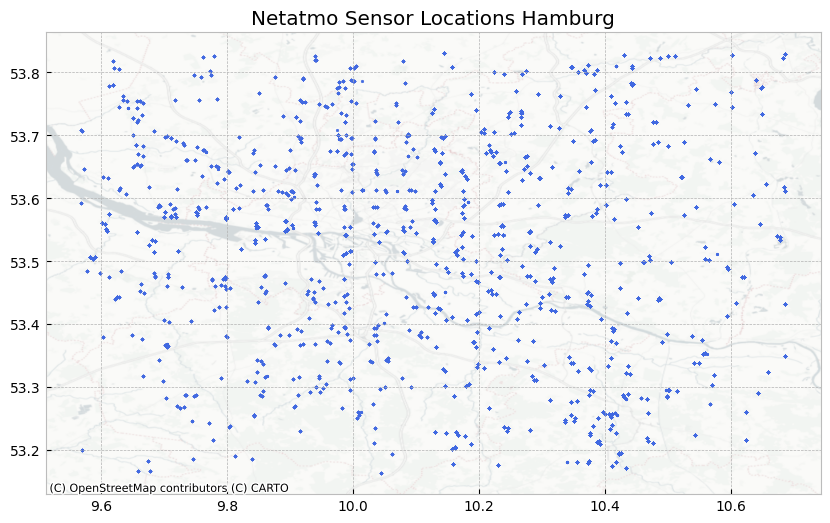
\includegraphics[width=1\textwidth]{images/netatmo_sensor_locations_hamburg.png}
    \caption{Sensor locations of Netatmo in Hamburg, Germany, as of 28.06.2023}
    \label{fig:netatmo sensor locations hamburg}

    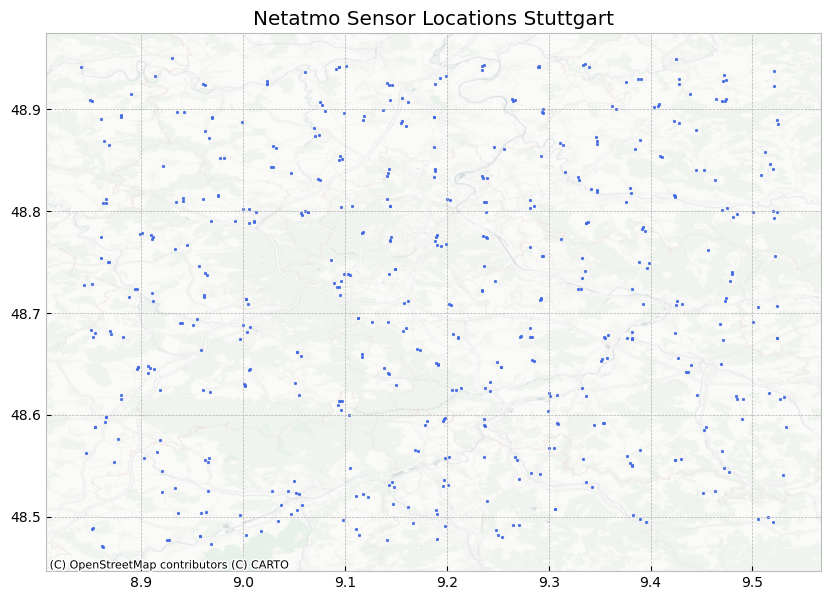
\includegraphics[width=1\textwidth]{images/netatmo_sensor_locations_stuttgart.png}
    \caption{Sensor locations of Netatmo in Stuttgart, Germany, as of 19.06.2023}
    \label{fig:netatmo sensor locations stuttgart}
\end{figure}

\subsubsection{Quality Considerations}

Netatmo sensors have a good measurement accuracy; however, due to the compact design, an aluminium housing, poor ventilation due to the small case, no dedicated radiation screen resulting in a proneness to radiative errors, and therefore overall slow sensor-response time~\cite{meier2017crowdsourcing, buchau2018modelling}, Netatmo weather stations have a systematic bias that influences data quality. Due to the uniformity of Netatmo sensors, e.g., all sensors are built in the same way, this bias could be corrected in the \gls{qc} step; however, this is not further explored in this work.

\subsection{Other Providers}

Other sources for crowdsourced weather station data include \gls{wow}~\footnote{\url{https://wow.metoffice.gov.uk/}, \textit{last accessed: 01.09.2023}} and Weather Underground~\footnote{\url{https://www.wunderground.com/}, \textit{last accessed: 01.09.2023}}.
\gls{wow} is a platform run by the UK Met Office, which is the UK's national weather service, and has a dense sensor coverage in the UK and the Netherlands as seen in figure~\ref{fig:wow sensor locations}.
Weather Underground is a commercial weather service which also provides a crowdsourced weather station network. Unfortunately, Weather Underground only provides an API for users with a registered weather station or other bulk download options for historical data. The website would allow for manual download of historical data, but this is not feasible for the amount of data needed in this work.

\begin{figure}[ht]
    \centering
    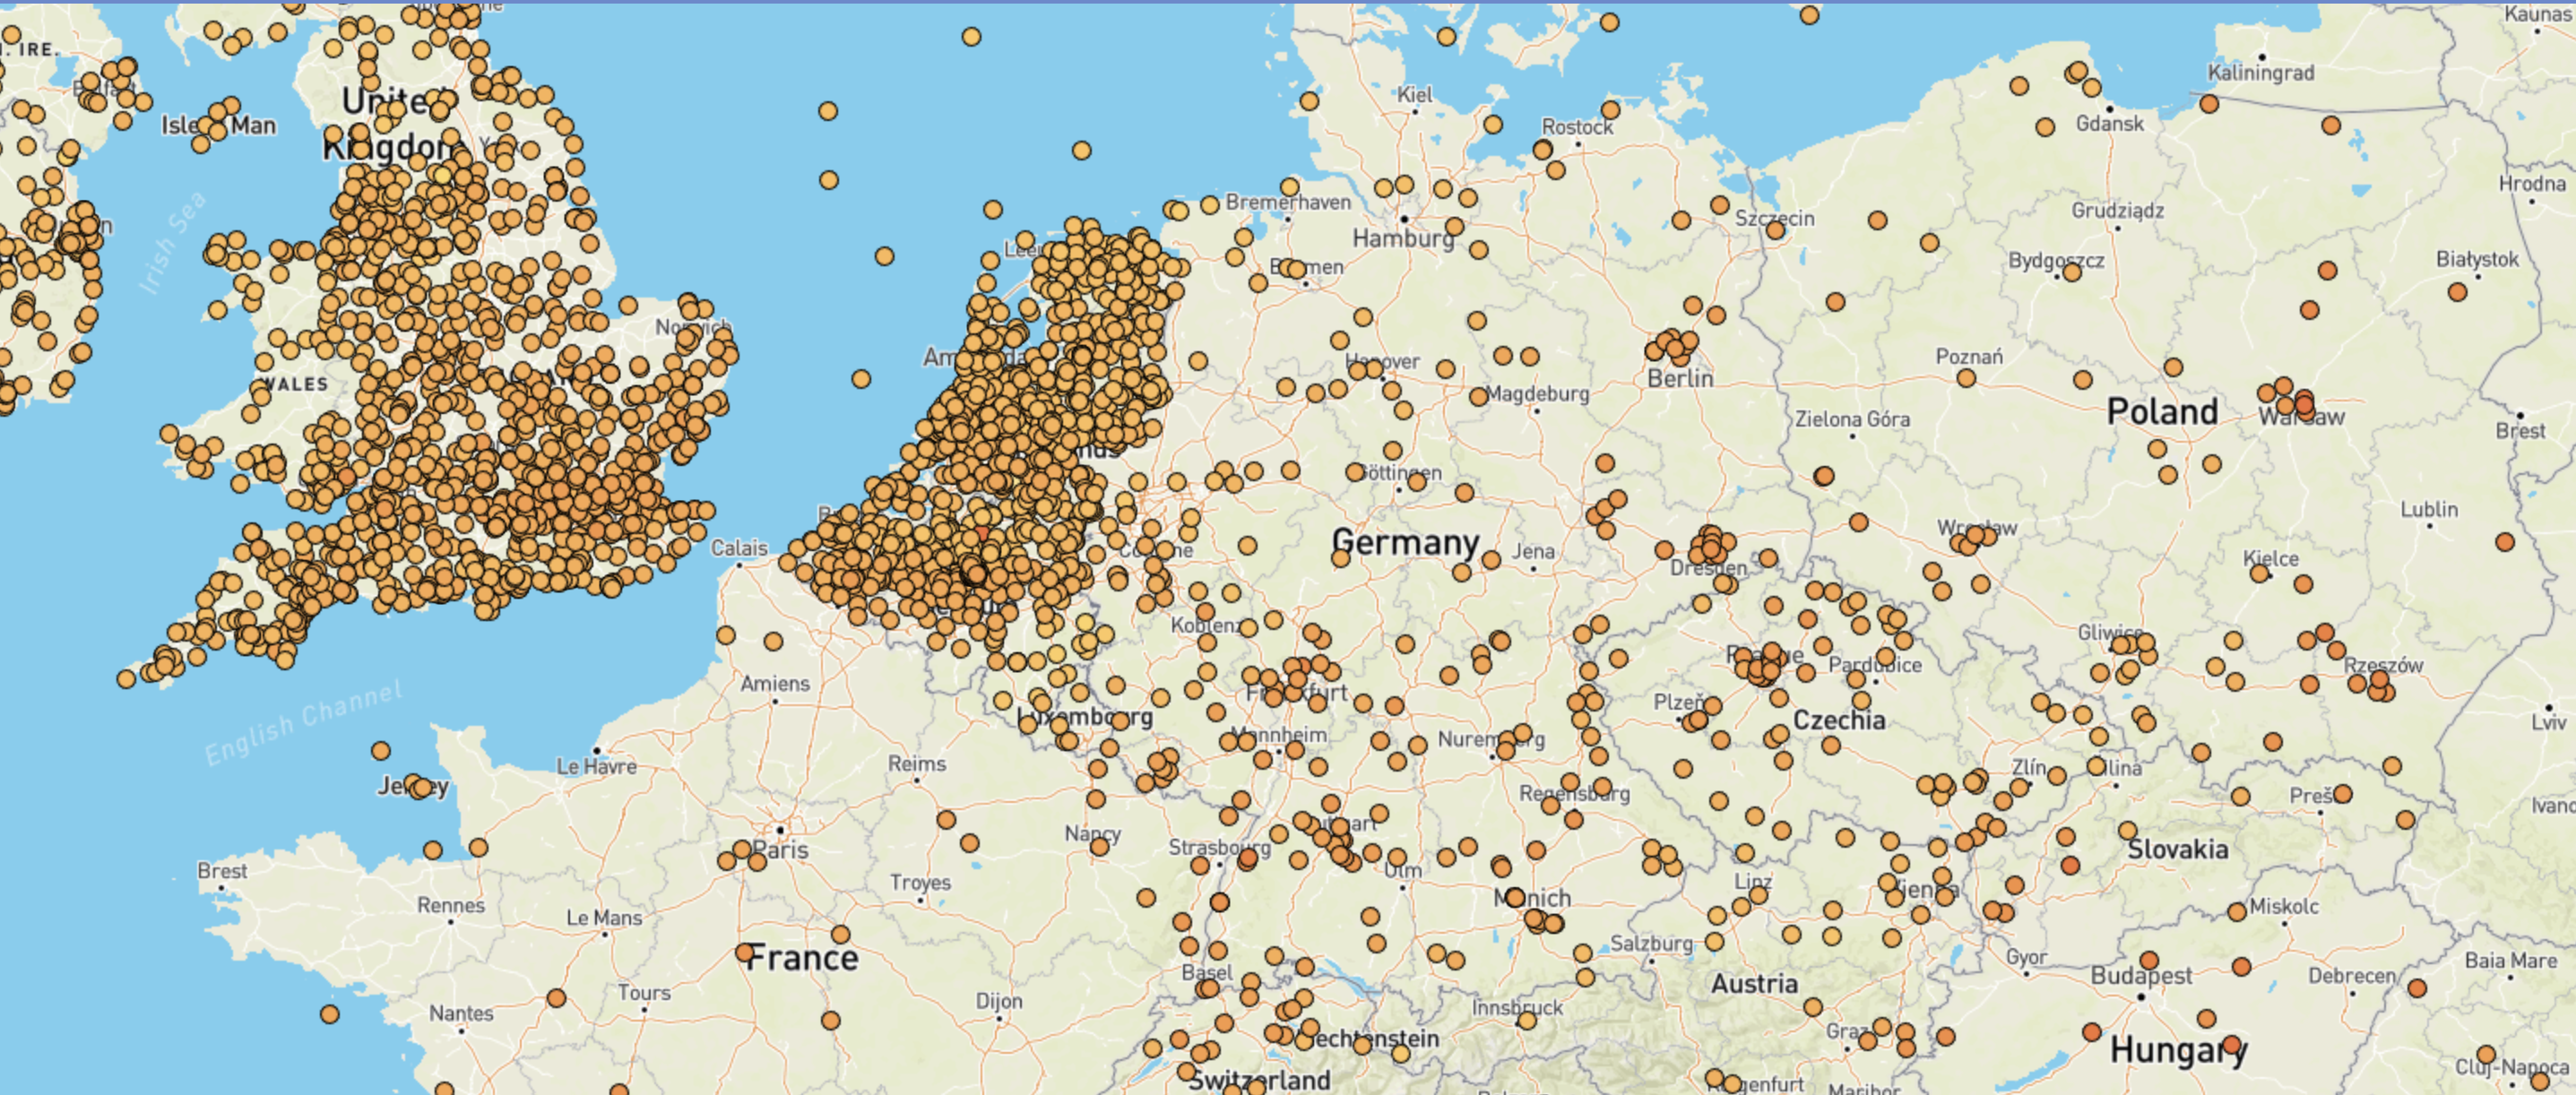
\includegraphics[width=1\textwidth]{images/wow_sensor_locations.png}
    \caption{Temperature sensor locations from \gls{wow}, accessed on 05.07.2023}
    \label{fig:wow sensor locations}
\end{figure}

\section{Reference Data Providers}

In order to add additional validation to crowdsourced weather data, reference data from (official) weather stations can be used. These weather stations should be setup according to current \gls{wmo} guidelines~\cite{wmo2018guide} to ensure high data quality. These standards are either achieved by official weather services, or by institutions such as universities whose sensors are maintained by experts.

\subsection{DWD}

The \gls{dwd} has many objectives that are defined by the \gls{dwd}-law in Germany. Its tasks include meteorological and climatological monitoring of the atmosphere, meteorologically securing the airspace for civil aviation, monitoring the Maritim climate, and more. The \gls{dwd} operates a large monitoring network and publishes most of its data via its OpenData portal~\footnote{\url{https://opendata.dwd.de/}, last accessed 13.07.2023}.\\
The main advantages of the \gls{dwd} data are high data quality through reference instruments and proper setup according to \gls{wmo} guidelines~\cite{wmo2018guide}. The main disadvantage is the low spatial coverage of the data, as stations are sparsely distributed to measure the overall mesoscale climate, as seen in Figure~\ref{fig:dwd sensor locations germany}. Additionally, a lot of the public weather stations are located close to airports, which are usually located outside of cities, and therefore not suitable for measuring urban microclimates.

\begin{figure}[ht]
    \centering
    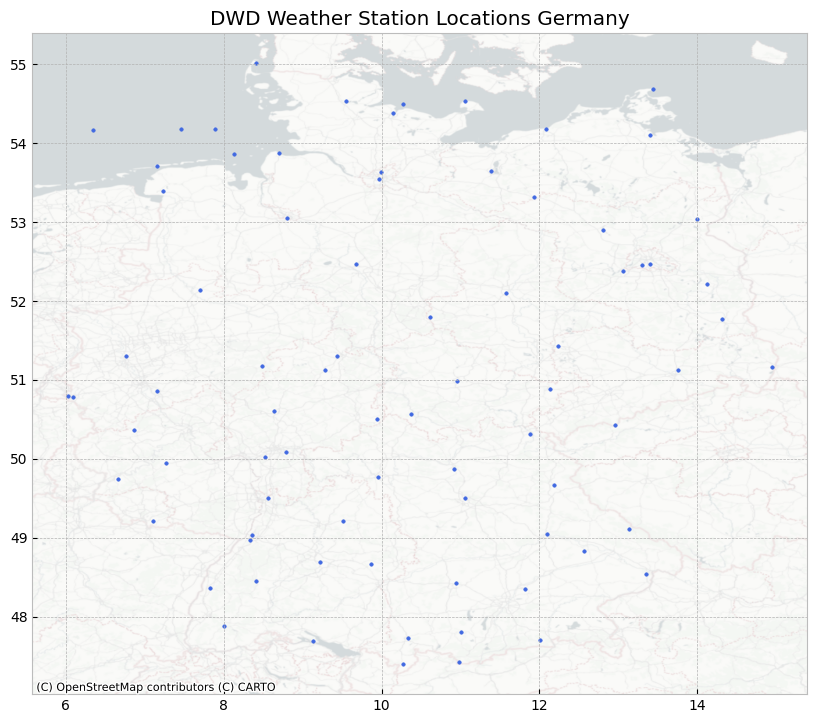
\includegraphics[width=1\textwidth]{images/dwd_weather_station_locations_germany.png}
    \caption{\gls{dwd} Weather Station Locations in Germany, \url{https://opendata.dwd.de/climate_environment/CDC/observations_germany/climate/subdaily/standard_format/KL_Standardformate_Beschreibung_Stationen.txt}, accessed 28.06.2023}
    \label{fig:dwd sensor locations germany}
\end{figure}

\subsubsection{Urban Climate Stations}

Next to the official weather stations, the \gls{dwd} also operates urban weather stations; however, there are currently only four stations in the following cities:

\begin{itemize}
    \item Berlin-Alexanderplatz, Berlin, Berlin
    \item Freiburg-Mitte, Freiburg, Baden-Württemberg
    \item Hannover-Nordstadt, Hannover, Niedersachsen
    \item Dresden-Neustadt, Dresden, Sachsen
\end{itemize}

The number of urban weather stations is planned to be gradually extended to reach 10 stations with the locations being primarily determined by the measurement objectives such as determining a city's maximum \gls{uhii}~\footnote{\url{https://www.dwd.de/EN/climate\_environment/climateresearch/climate\_impact/urbanism/urban\_heat\_island/urbanheatisland\_node.html}, \textit{last accessed: 01.09.2023}}. Due to the low number of weather stations, their data is not used in this work.

\subsubsection{Weather Radar}

The \gls{dwd} also operates a network of weather radars~\footnote{\url{https://www.dwd.de/DE/leistungen/radarprodukte/radarprodukte.html}, \textit{last accessed 12.07.2023, not available in english}} that are used to measure precipitation and wind speed. This data could be interesting in the context of air interpolation in order to detect precipitation events that have a mayor influence on humidity and temperature or to detect wind speeds that also play an important factor in dissipating heat and transporting it away from urban areas. Due to the limited scope of this work, this data is currently not used.

\subsection{Locally Operated Weather Stations}

Next to official weather services, many public and private institutions operate weather stations. The following section lists two examples of such institutions, the Meteorological Institute of the University of Hamburg and the Office for Environmental Protection of the City of Stuttgart.

\subsubsection{University of Hamburg – Meteorological Institute}

In Hamburg the Meteorological Institute of the University of Hamburg addresses local climate concerns, supports many projects, and support decision makers relating climatic concerns. One of its projects is the Hamburg Urban Soil Climate Observatory (HUSCO) which operates multiple urban climate weather stations that measure \gls{ta} at 2m height as well as many other parameters including soil temperatures and conditions. In the current scope of this work we do not use data from this project; however, it could be a good reference point especially in the context of 2m \gls{ta} for \gls{cuhi} detection and wanted to mention it here.

\begin{figure}[ht]
    \centering
    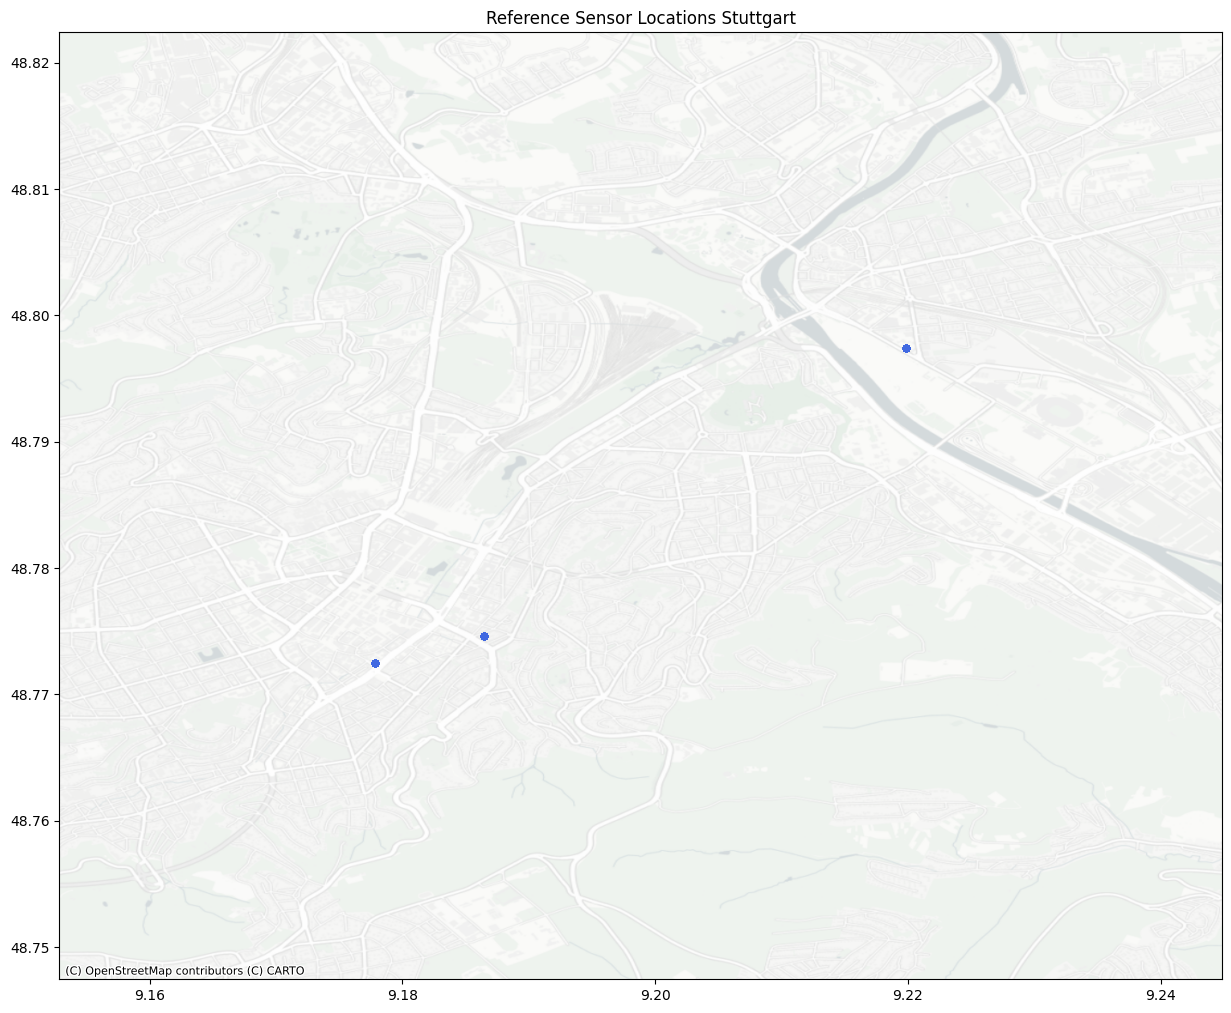
\includegraphics[width=1\textwidth]{images/afu_stuttgart_sensor_locations.png}
    \caption{Weather Station Locations in Stuttgart, \url{https://www.stadtklima-stuttgart.de/}, \textit{last accessed: 10.08.2023}}
    \label{fig:afu weather station locations}
\end{figure}

\subsubsection{City of Stuttgart – Office for Environmental Protection}

The Office for Environmental Protection of the city of Stuttgart has the goal of monitoring the climate in Stuttgart and the surrounding area and improve the living conditions of the citizens. The main focus of the office is on air quality, noise, and (urban) climate. It operates several weather stations in the city of Stuttgart, which are shown in Figure~\ref{fig:afu weather station locations}. The data from these stations is published directly on the website, a detailed quality assessment is given, and reference grade sensors are used. Unfortunately, the stations are mounted on top of building, e.g., 20-23m above ground, which is not ideal for measuring urban microclimates as the \gls{ta} is several degrees cooler than directly on the ground. This example underlines the importance of proper sensor placement and meta-data documentation. The data from the weather stations could be corrected using the \gls{dwd} reference station nearby; however, uncorrected, the \gls{ta} cannot be used to validate the crowdsourced data. Due to the high placement, other measurements such as wind direction and speed could be used to get a good estimation of the overall climate in the city; however, not on the microscale.

\section{Remote Sensing Data Providers}

\subsubsection{Remote Sensing}
\label{subsec: remote sensing}

In comparison to stationary sensors that are installed directly in the environment they are observing, remote sensing describes the process of observing a target environment from afar~\cite{campbell2011introduction}. In climatology, remote sensing is used to collect meteorological data via satellites, planes, or balloons by either capturing image data that can be used to identify things like cloud and land coverage, by measuring passive radiation, or by actively sending out microwaves or using LiDAR to detect features such as \gls{lst}. Remote sensing comes with its own set of advantages and challenges.\\
The major upside of sensors moving way above ground is the high spatial coverage, that allows for meso- and planetary-scale analysis of weather phenomena. Another upside is the great data availability, as many satellite providers (e.g., NASA, ESA, etc.) publish their satellite data. This creates many research opportunities and services directly relying on these measurements.\\
Remote sensing also comes with certain downsides. The primary downside is the low spatio-temporal resolutions. Weather satellites usually are not orbit-stationary and move around earth on a predetermined orbit. Consequently, satellites only pass over each individual area a couple times a day, making real-time applications for currently unobserved areas impossible. Additionally, the spatial resolution can be too low for micro-/local-scale analysis, with typical \gls{lst} resolution spanning from 1 km$^{2}$ to tens or even hundreds of km$^{2}$ per data point/grid field. In the atmosphere, there is also a lot of environmental noise, like radiation, that can have a negative influence on the measurement accuracy. Another disturbing factor can be clouds or other types of particles like rain that absorb radiation/microwaves sent from the sensors, making measuring under cloudy/rainy conditions either impossible. There exist methods to estimate values instead, relying on outgoing radiation from the surface; however, these approaches are usually less accurate. These restrictions highly depend on the sensor used, as different sensors use different sensors use different technologies, e.g., microwaves with different wave lengths or higher resolution sensors.

\subsection{Google Earth Engine}

\gls{gee} is a science data and analysis platform that allows users to work with and transform massive datasets with remote sensing data that are available as OpenSource~\cite{gorelick2017google}. Remote sensing data in this work is processed and obtained via this platform and used datasets are cited. Datasets available on \gls{gee} are not published by Google itself but from institutions such as NASA, ESA, or the European Union.

\section{Quality Control}
\label{sec:quality control}

\gls{qc} is an essential step in the process of data analysis and preparation. The goal is to identify and remove outliers in the data that are due to placement errors of sensors, sensor malfunctions, sensor inaccuracies or other errors. In the context of \gls{pws}, weather stations are placed and maintained by non-professionals, making \gls{qc} even more important. One of the main challenges in the context of (hyper-) local urban \gls{ta} data is to not flag data as outliers that is representative of the local climate in case of extreme temperature, e.g., heat islands, and at the same time identify erroneous or wrongly placed sensors, e.g., too close to walls, in direct sunlight, indoors, etc. Additionally, current \gls{pws} networks do not track sufficient metadata on the sensor placement, e.g., sensor height, which also plays an important role in protecting the privacy of citizens and not exposing too accurate sensor locations.\\
Due to the popularity of Netatmo weather station data in research due to high spatio-temporal resolution, there are several software libraries available that help simplify and automate the \gls{qc} process. These tools were primarily developed for Netatmo temperature data; however, CrowdQC and TITAN can also be used for other nearly-normally distributed data sources~\cite{hahn2022observations}. The following tools are available:

\begin{itemize}
    \item CrowdQC (R package~\footnote{\url{https://doi.org/10.14279/depositonce-6740.3}})
    \item CrowdQC+~\cite{fenner2021crowdqc+} (R package~\footnote{\url{https://github.com/dafenner/CrowdQCplus}, \textit{last accessed: 01.09.2023}})
    \item TITAN (R package~\footnote{\url{https://github.com/metno/TITAN}, \textit{last accessed: 01.09.2023}})
    \item NetatmoQC (Python 3 package~\footnote{\url{https://source.coderefinery.org/iOBS/wp2/task-2-3/netatmoqc}, \textit{last accessed: 01.09.2023}})
\end{itemize}

In this work, CrowdQC+ is used for \gls{qc} as it offers improvements and bug fixes compared to CrowdQC. It's an open-source software library written in R, a popular programming language for statistical applications. The data needs to be in the following format:

\begin{itemize}
    \item \textit{p\_id}: The unique ID of the station
    \item \textit{time}: The time of the measurement
    \item \textit{ta}: The \gls{ta} in degree Celsius
    \item \textit{lon}: The longitude of the station
    \item \textit{lat}: The latitude of the station
    \item \textit{z}: The height of the station in meters, optional
\end{itemize}

The CrowdQC+ library implements the following required steps of \gls{qc}:\ Metadata Check, Distribution Check, Data Validity, Temporal Correlation, Spatial Buddy Check. There are also the following optional steps available, that are currently not used: Temporal Interpolation, Daily Validity, Validity in Time Period, and Correction for Time Constant.
The steps used in this work are shown and explained in Table~\ref{tab: qc_steps}, including the number of data and stations available after each step.\\
In their own study, CrowdQC+ kept 47.1\% and 69.2\% of data after steps m1-5, and only 20.7\% and 29.5\% after steps o1-o3, for the cities Amsterdam and Toulouse respectively~\cite{fenner2021crowdqc+}, given default parameters. In that setting, CrowdQC kept more data with 41.0\% in Amsterdam and 54.9\% in Toulouse. In this work, CrowdQC+ is used with default parameters excluding height validation, as this data was not available for almost all sensors. Additionally, only the first 5 required steps are used, as the optional steps are not needed for the interpolation. The input data for CrowdQC+ also needs have the same temporal resolution and intervals.\\
In this study, we use a 10 min interval to have a high temporal resolution and use the default parameters except excluding the heigh check due to the missing values. Important to note here, that in the following, only the \gls{ta} is validated and no other measurements such as pressure or humidity. CrowdQC+ could be used for other approximately normally distributed features; however, there hasn't been more specific research in this direction. We assume that a station that seems to be setup correctly and produces good \gls{ta} measurements, also captures the other measurements correctly for simplicity reasons.

\begin{figure}[htp]
    \centering
    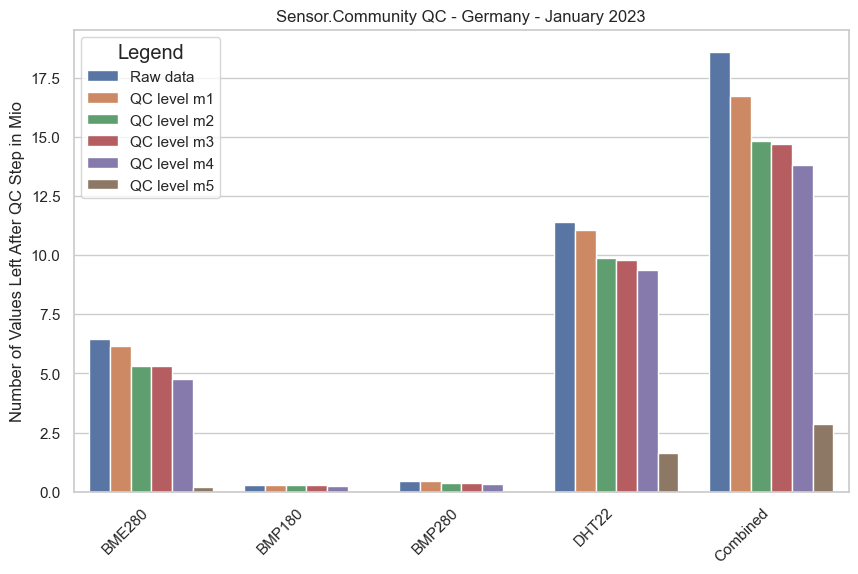
\includegraphics[width=1\textwidth]{images/sensor_community_qc_january_23.png}
    \caption{QC Results for Sensor.Community Data for Germany, January 2023}
    \label{fig:qc sensor community jan 23}

    \centering
    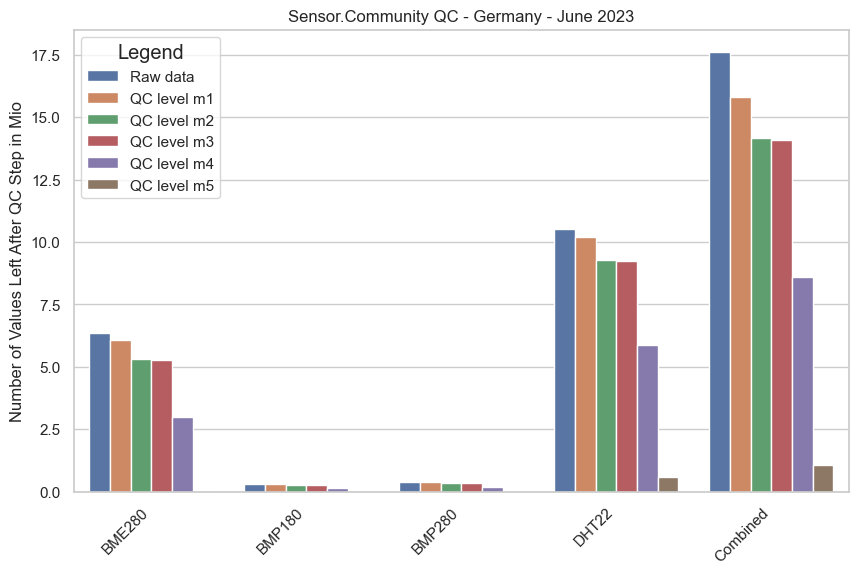
\includegraphics[width=1\textwidth]{images/sensor_community_qc_june_23.png}
    \caption{QC Results for Sensor.Community Data for Germany, June 2023}
    \label{fig:qc sensor community june 23}
\end{figure}

\subsection{Quality Control for Sensor.Community}

For Sensor.Community, we can see several interesting things for the \gls{ta}. The first is, that in January 2023 less data is lost due to \gls{qc} compared to June 2023. This could be to the fact, that in colder environments with less solar radiation, sensor placement, for example close to buildings, has less of an influence. In comparison, June 2023 had many hotter days, therefore it could be that more extreme readings are flagged as outliers. We can also see that Sensor.Community loses a lot of stations in step m4 in June 2023 compared to January 2023, which is the temporal correlation with the median of all stations. This could also be due to a higher temperature difference across Germany, therefore comparing smaller areas could be beneficial for this. We can also see, that the m5 check, which is the buddy check with surrounding stations, also removes a lot of stations which could be due to the low station density.\\
The CrowdQC+ library can theoretically be used to validate other near-normally distributed variables; however, this could change the way the \gls{qc} step parameters should be set and changed from the default. For the \gls{ta}, the default parameters as proposed by the library were used. Due to the limited scope, for other readings, e.g., relative humidity and atmospheric pressure, we simply remove default values. As an improvement, for other variables a more sophisticated \gls{qc} process should be used. In addition, due to the low sensor density and the fact, that all types of sensors used are good \gls{lcs}s, we simply combine all sensor readings after \gls{qc} step m5 into one dataset and ignore the sensor type.\\
After the \gls{qc} process, the Sensor.Community sensor locations left are shown in~\ref{fig:qc sensor community germany june 23}. In this figure we can see, that there are many sensors left in Stuttgart, Hamburg, Munich, and some in Cologne. Due to \gls{dwd} stations only being present in Hamburg and Stuttgart, those two areas are candidates for further usage.

\begin{figure}[ht]
    \centering
    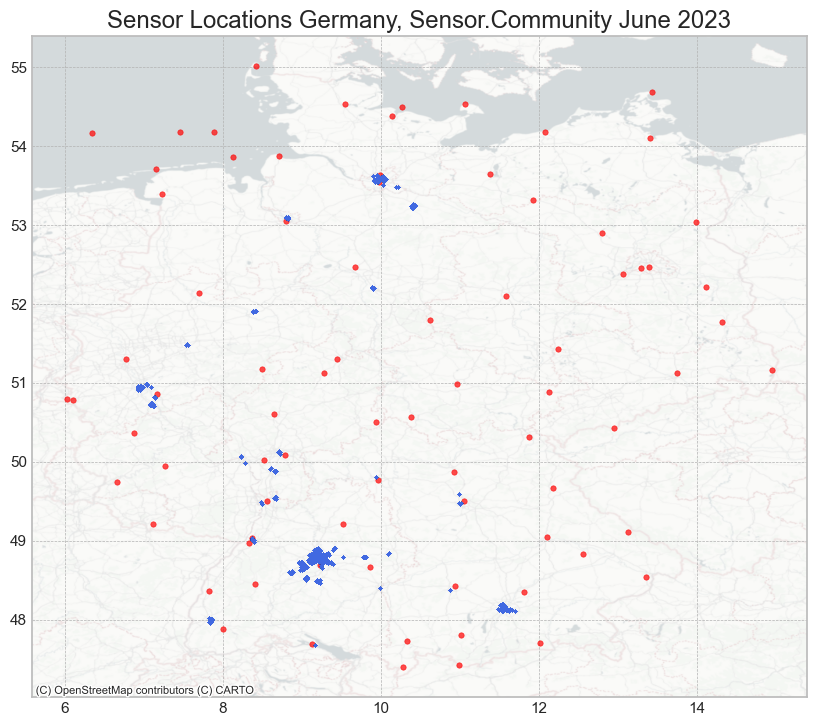
\includegraphics[width=1\textwidth]{images/sensor_community_locations_germany_after_qc_june_23.png}
    \caption{QC Results for Sensor.Community for Germany, June 2023}
    \label{fig:qc sensor community germany june 23}
\end{figure}

\begin{sidewaystable}
\label{tab: qc_steps}
\caption{Quality Control Steps of CrowdQC+}
\resizebox{\textwidth}{!}{
\begin{tabular}{lllllll}
\hline
\textbf{}         & \textbf{Id} & \textbf{Name of Step}        & \textbf{Functionality}                                                                                                                                                                                                                                                        & \textbf{\% of Data} & \textbf{Num Stations} & \textbf{Num Values} \\ \hline
\textbf{Required} &             &                              &                                                                                                                                                                                                                                                                               &                                                                                    &                                                                                         &                                                                  \\
                  & m1          & Metadata Check               & \begin{tabular}[c]{@{}l@{}}Validates longitude and latitude values and removes stations with\\ identical values. Mainly aims to remove stations with default values\\ from locations from IP addresses due to improper configuration\\ by the end-user\end{tabular}           & 97.40\%                                                                            & 1077                                                                                    & 2.082.283                                                        \\
                  & m2          & Distribution Check           & \begin{tabular}[c]{@{}l@{}}Primarily targets radiative error that lead to unrealistic high ta\\ values and sensors installed indoors\end{tabular}                                                                                                                             & 86.50\%                                                                            & 1041                                                                                    & 1.849.247                                                        \\
                  & m3          & Data Validity                & \begin{tabular}[c]{@{}l@{}}Checks values of stations that did not pass m2. If more than 20\%\\ of data didn't pass the check, the station is considered to be faulty\\ and is removed\end{tabular}                                                                            & 85.20\%                                                                            & 845                                                                                     & 1.821.479                                                        \\
                  & m4          & Temporal Correlation         & \begin{tabular}[c]{@{}l@{}}Checks the temporal correlation between each station and the\\ median of all stations for a specified period of time, default 1\\ month. Targets indoor stations that have weak temporal\\ correlation to the median of all stations.\end{tabular} & 79.90\%                                                                            & 829                                                                                     & 1.708.061                                                        \\
                  & m5          & Spatial Buddy Check          & \begin{tabular}[c]{@{}l@{}}Neighbourhood-based check to identify outliers within a specific\\ area. Primarily targets radiation errors with too high ta values.\\ Defaults to radius of 3000m and 5 neighbours.\end{tabular}                                                  & 31.53\%                                                                            & 466                                                                                     & 674.004                                                          \\
\textbf{Optional} &             &                              &                                                                                                                                                                                                                                                                               &                                                                                    &                                                                                         &                                                                  \\
                  & o1          & Temporal Interpolation       & \begin{tabular}[c]{@{}l@{}}Step to interpolate missing values in the time-series of each\\ station to increase data availability\end{tabular}                                                                                                                                 & -                                                                                  & -                                                                                       & -                                                                \\
                  & o2          & Daily Validity               & Verifies robust calculations of daily values                                                                                                                                                                                                                                  & -                                                                                  & -                                                                                       & -                                                                \\
                  & o3          & Validity in Time Period      & Checks if enough values are available in a given time frame                                                                                                                                                                                                                   & -                                                                                  & -                                                                                       & -                                                                \\
                  & o4          & Correction for Time Constant & \begin{tabular}[c]{@{}l@{}}Sensors have different times that they respond to ta changes.\\ Due to Netatmo design flaws, a\\ constant correction for all stations can be applied.\end{tabular}                                                                                 & -                                                                                  & -                                                                                       & -                                                                \\ \hline
\end{tabular}}
\vspace{1ex}

{\raggedright This table shows the \gls{qc} steps used in this work from the CrowdQC+ library, including the \% of data available after each step, the number of stations available and the number of values left after each step. Optional steps are currently not used. \par}
\end{sidewaystable}

\begin{figure}[htp]
    \centering
    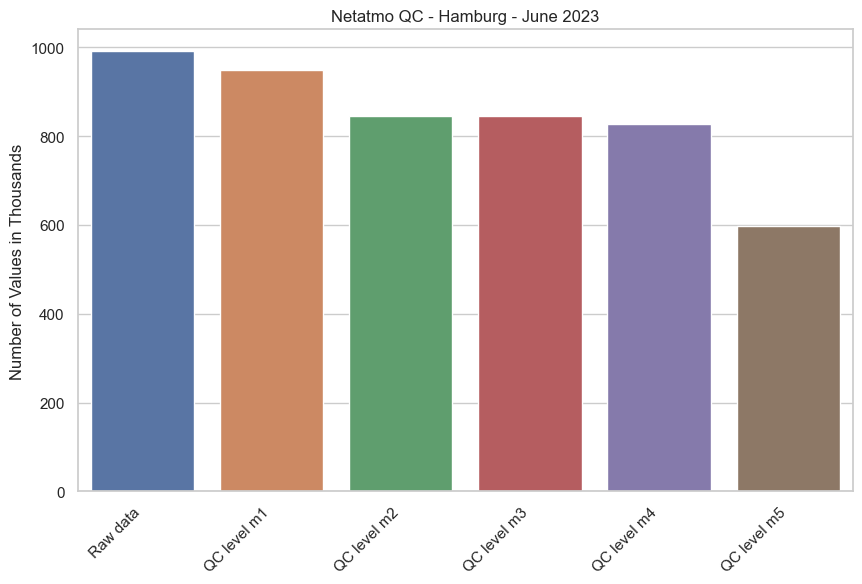
\includegraphics[width=1\textwidth]{images/netatmo_qc_june_23.png}
    \caption{\gls{qc} Result Statistics for Netatmo Data for Hamburg, June 2023}
    \label{fig:qc netatmo june 23}
\end{figure}

\subsection{Quality Control for Netatmo}

The \gls{qc} results for Netatmo stations in Hamburg during June 2023 can be found in~\ref{fig:qc netatmo june 23} which shows the absolute values of sensor readings available after each step including the overall available data as `Raw data' before \gls{qc} which is 1.026.721 rows.
After \gls{qc} 60.24\% of Netatmo data is still available in Hamburg (so a loss of 39.76\%). The amount of data kept is in line with comparable cities as tested by CrowdQC+'s study which kept 47.1\% and 69.2\% for the cities Amsterdam and Toulouse respectively after steps m1-m5~\cite{fenner2021crowdqc+} as mentioned above. Another comparison can be made to the study by Meier et al.\ which kept 47\% of Netatmo data in Berlin after \gls{qc} with CrowdQC~\cite{meier2017crowdsourcing}.
It is interesting to note that stations directly next to water seem to be removed proportionally more often. This could be due to higher variability of wind close to water~\cite{ho2014mapping} which can result in higher prediction errors.\\
A station is not necessarily removed at all times, only if it shows outliers for a certain period after \gls{qc} step m3, maybe due to improper setup. The difference between day and night for an example day of 19.06.2023 can be found in Appendix~\ref{appendix: netatmo}  Figure~\ref{fig:qc netatmo hamburg before after m5}.

\section{Feature Engineering}
\label{sec:feature_engineering}

The goal of feature engineering is to create features from the available data that can be used as input for the machine learning models. Based on the features, different models can be used for completely different tasks such as interpolation vs.\ extrapolation. The process includes the selection of features, the extraction of features from the raw data, and the transformation of features into a format that can be used by the machine learning models which could include scaling and/or normalization. Especially in the context of \gls{ta} interpolation, a lot of domain knowledge is required to select the right features and model correlations between them correctly. The target feature in this work is the \gls{ta} at canopy height, e.g., 2m height so that \gls{cuhi}s could be detected when using these trained interpolation models. Alternatively, the target temperature could also be adapted to be measured at another height or be exchanged based on the use-case.\\
The input features are a combination of sensor readings from \gls{pws} networks such as Sensor.Community and Netatmo, satellite data such as land cover and vegetation health or \gls{lst}, and additional meta data such as soil conditions, zoning plans, or locations of sensors. The goal of this section is to give an overview of the different features that can be used for \gls{ta} interpolation and discuss several highly important features that are especially relevant in the context of urban microclimate based on related studies. Important questions are: 1. What features are there and how can they be measured/sourced from? 2. How do features for the 2 use cases, e.g., single station interpolation vs.\ areal interpolation, differ? 3. How do we handle \gls{qc} outputs? 4. How do we deal with correlations between inputs so that we do not introduce bias into our models?

\subsection{Feature Engineering Pipelines and Automation}

Before looking at available features and features used in related work, we quickly return to the topic of Smart City and how to integrate different data sources and automate the feature engineering process. A popular solution for production-ready \gls{ml} applications is the use of pipelines that streamline the data pre-processing, feature engineering, potential re-training, and prediction processes. Luckily, all data-sources previously mentioned have APIs or offer download options to get access to recent sensor readings. Next to the \gls{ta} readings which can be sourced from Netatmo, Sensor.Community, and/or the \gls{dwd}, other features are also important to get good prediction, as suggested by Zumwald et al.\ where \gls{ta} at 2m only explained 33\% of the prediction~\cite{zumwald2021mapping}, such as remote sensing information, that for example could be sourced from \gls{gee}.\\
The actual sensor readings come directly from the sensing layer, in which different external sources could be integrated via API, so that virtual sensors are created that are directly available for example via a overlay network such as SkipNet. In this work, we do not take advantage of other solutions but instead source data directly via API or archives to make a historical data analysis instead of testing real-time applications. After transporting this information via the transportation layer to the data-management layer, the service layer can consume the data streams. An \gls{ta} interpolation service could then be placed in the service layer for areal interpolation. This service could then be used for areal interpolation to provide fine-granular \gls{ta} maps/grids. The use-case of single station interpolation, for example in combination with moving sensors might be better located in the sensing layer as a virtual sensor; however, challenges would be the dependency on other sensors which might have different sampling intervals.\\
In this work, we only take advantage of sklearn pipelines~\footnote{\url{https://scikit-learn.org/stable/modules/generated/sklearn.pipeline.Pipeline.html}, \textit{last accessed: 27.08.2023}} in a limited fashion for the actual training and testing process to automatically include scaling and cross-validation and rely on many manual steps to download the data, do pre-processing and \gls{qc}, and finally extract features and train \gls{ml} models.

\subsection{Feature Overview}

In the following sections, we look at available features for the use-case of \gls{ta} interpolation.

\subsubsection{Essential Climate Variables}

\gls{ecv}s are a list of currently 50 variables that are proposed by the \gls{wmo} to measure climate and climate change. The \gls{wmo} regularly publishes updates on which climate variables to use and how to measure them~\cite{wmo2018guide}. \gls{ecv}s are generally more focused on measuring climate on a global scale; however, they also contain many variables that are relevant for urban microclimate, such as \gls{ta} and land cover. There are three categories of \gls{ecv}s, namely Atmosphere, Land, and Ocean. And overview of the \gls{ecv}s can be found online~\footnote{\url{https://gcos.wmo.int/en/essential-climate-variables/table}, \textit{last accessed: 08.08.2023}}.\\
Next to official \gls{wmo} suggestions, other institutions such as the Integrated Climate Data Centre (ICDC) from the University of Hamburg (UHH) also suggest variables to measure climate~\footnote{\url{https://www.cen.uni-hamburg.de/icdc/data.html}, \textit{last accessed: 27.08.2023}}. Table~\ref{tab:icdc datset parameters} shows the available parameters for which datasets are available.

\begin{table}[ht]
    \footnotesize
    \centering
    \begin{tabular}{|c|c|}
        \hline
        \textbf{Category} & \textbf{Parameters} \\
        \hline
        \multirow{9}{*}{Atmospheric Data} & Air Temperature \\
        & Pressure \\
        & Wind \\
        & Precipitation \\
        & Clouds \\
        & Aerosols \\
        & Humidity \\
        & Radiation \\
        & Climate Indices \\
        \hline
        \multirow{7}{*}{Ocean} & Water Temperature \\
        & Wave Height (SSH) \\
        & Salt Content \\
        & Tide \\
        & Ocean Colour \\
        & Climatology \\
        & Ocean Currents \\
        \hline
        \multirow{8}{*}{Ice/Snow} & Sea Ice Coverage \\
        & Sea Ice Thickness \\
        & Sea Ice Type \\
        & Snow Thickness (Ice) \\
        & Snow Water Equivalent (SWE) \\
        & Land Snow Cover \\
        & Glacier Thickness \\
        & Melting Ponds \\
        \hline
        \multirow{7}{*}{Land} & Albedo \\
        & Surface Temperature \\
        & Vegetation \\
        & Soil Moisture \\
        & Topography \\
        & Short-wave Radiation \\
        & Permafrost \\
        \hline
        \multirow{1}{*}{Society} & Social Science Parameters \\
        \hline
    \end{tabular}
    \caption{ICDC Dataset Parameters}
    \label{tab:icdc datset parameters}
\end{table}

\begin{table}[htp]
    \footnotesize
    \centering
    \begin{tabular}{|lll|lll|}
    \hline
    \textbf{}                & \textbf{Variables (Units)}                                                                   & \multicolumn{1}{c}{\textbf{\begin{tabular}[c]{@{}c@{}}Acquisition\\ Source\end{tabular}}} & \textbf{}                & \textbf{Variables (Units)}                                                            & \multicolumn{1}{c|}{\textbf{\begin{tabular}[c]{@{}c@{}}Acquisition\\ Source\end{tabular}}} \\ \hline
    \rowcolor[HTML]{EFEFEF} 
                            & \textbf{Vegetation Index}                                                                    &                                                                                           &                          & \textbf{Radiation Index}                                                              &                                                                                            \\
                            & \begin{tabular}[c]{@{}l@{}}Normalized Difference Vegetation\\ Index (\gls{ndvi})\end{tabular}      & Landsat 8                                                                                 &                          & Spectral Radiance                                                                     & Landsat 8                                                                                  \\
                            & Enhanced Vegetation Index (EVI)                                                              & Landsat 8                                                                                 &                          & Emissivity                                                                            & Landsat 8                                                                                  \\
                            & \begin{tabular}[c]{@{}l@{}}Soil Adjusted Vegetation Index\\ (SAVI)\end{tabular}              & Landsat 8                                                                                 &                          & \begin{tabular}[c]{@{}l@{}}Tasseled Cap Transformation\\ Brightness\end{tabular}      & Landsat 8                                                                                  \\
                            & \begin{tabular}[c]{@{}l@{}}Tasseled Cap Transformation\\ Greenness (GVI)\end{tabular}        & Landsat 8                                                                                 & \cellcolor[HTML]{EFEFEF} & \cellcolor[HTML]{EFEFEF}\textbf{Building Index}                                       & \cellcolor[HTML]{EFEFEF}                                                                   \\
                            & Density of Low Vegetation                                                                    & LiDAR                                                                                     &                          & \begin{tabular}[c]{@{}l@{}}Normalized Difference Buit-Up\\ Index (NDBI)\end{tabular}  & Landsat 8                                                                                  \\
                            & Density of Medium Vegetation                                                                 & LiDAR                                                                                     &                          & Urban Index (UI)                                                                      & Landsat 8                                                                                  \\
                            & Density of High Vegetation                                                                   & LiDAR                                                                                     &                          & Index-based Built-Up Index (IBI)                                                      & Landsat 8                                                                                  \\
    \cellcolor[HTML]{EFEFEF} & \cellcolor[HTML]{EFEFEF}\textbf{Water Presence Index}                                        & \cellcolor[HTML]{EFEFEF}                                                                  &                          & Building Density                                                                      & LiDAR                                                                                      \\
                            & \begin{tabular}[c]{@{}l@{}}Modified Normalized Difference\\ Water Index (MNDWI)\end{tabular} & Landsat 8                                                                                 & \cellcolor[HTML]{EFEFEF} & \cellcolor[HTML]{EFEFEF}\textbf{Urban Morphology}                                     & \cellcolor[HTML]{EFEFEF}                                                                   \\
                            & \begin{tabular}[c]{@{}l@{}}Normalized Difference Water\\ Index (NDWI)\end{tabular}           & Landsat 8                                                                                 &                          & Sky View Factor                                                                       & LiDAR                                                                                      \\
    \cellcolor[HTML]{EFEFEF} & \cellcolor[HTML]{EFEFEF}\textbf{Bare Soil Index}                                             & \cellcolor[HTML]{EFEFEF}                                                                  &                          & \begin{tabular}[c]{@{}l@{}}Standard Deviation (STD) of\\ Building Height\end{tabular} & \begin{tabular}[c]{@{}l@{}}Local\\ Authority\end{tabular}                                  \\
                            & \begin{tabular}[c]{@{}l@{}}Normalized Difference Bareness\\ Index (NDBaI)\end{tabular}       & Landsat 8                                                                                 & \cellcolor[HTML]{EFEFEF} & \cellcolor[HTML]{EFEFEF}\textbf{Moisture Index}                                       & \cellcolor[HTML]{EFEFEF}                                                                   \\
                            & Bare Soil Index (BI)                                                                         & Landsat 8                                                                                 &                          & \begin{tabular}[c]{@{}l@{}}Tasseled Cap Transformation\\ Index\end{tabular}           & Landsat 8                                                                                  \\
                            & \begin{tabular}[c]{@{}l@{}}Enhanced Built-Up and Bareness\\ Index (EBBI)\end{tabular}        & Landsat 8                                                                                 &                          & \begin{tabular}[c]{@{}l@{}}Normalized Difference Moisture\\ Index (NDMI)\end{tabular} & Landsat 8                                                                                  \\
                            & Density of Bare Soil                                                                         & LiDAR                                                                                     &                          &                                                                                       &                                                                                            \\ \hline
    \end{tabular}
    \caption{Indexes used by Alonso and Renard~\cite{alonso2020new} to predict \gls{ta}.}
    \label{tab:alonso_indexes}

    \begin{tabular}{|llll|}
    \hline
    \textbf{Variable}          & \textbf{Data source}                                                 & \textbf{Data type} & \textbf{Spatial resolution} \\ \hline
    Red                        & \begin{tabular}[c]{@{}l@{}}Landsat 7,8 and\\ Sentinel 2\end{tabular} & Open source        & L: 30m, S: 10m             \\
    Green                      &                                                                      &                    &                            \\
    Blue                       &                                                                      &                    &                            \\
    Near infrared              &                                                                      &                    &                            \\
    Short-wave infrared 1      &                                                                      &                    & L: 30m, S: 20m             \\
    Short-wave infrared 2      &                                                                      &                    &                            \\
    \gls{ndvi}                       &                                                                      &                    & L: 30m, S: 10m             \\
    IBI                        &                                                                      &                    & L: 30m, S: 20m             \\
    LST                        & Landsat 7,8                                                          &                    & 30m                        \\
    Elevation above sea        & STRM                                                                 &                    & 30m                        \\
    Terrain aspect             &                                                                      &                    &                            \\
    Terrain slope              &                                                                      &                    &                            \\
    Terrain ruggedness         &                                                                      &                    &                            \\
    CHM                        & LiDAR                                                                & Closed source      & 1m                         \\
    CHM slope                  &                                                                      &                    &                            \\
    CHM aspect                 &                                                                      &                    &                            \\
    CHM shadow/SVI             &                                                                      &                    &                            \\
    Building height            & \begin{tabular}[c]{@{}l@{}}LiDAR + building\\ footprint\end{tabular} &                    &                            \\
    Building height sd 1-4m    &                                                                      &                    &                            \\
    Building height sd 4-20m   &                                                                      &                    &                            \\
    Building height sd 20-100m &                                                                      &                    &                            \\
    Fractional tree cover      & \begin{tabular}[c]{@{}l@{}}LiDAR + ortho-\\ photo\end{tabular}       &                    &                            \\
    Tree height                &                                                                      &                    &                            \\
    Distance to coast          & Global water occurrence                                              & Open source        & 30m                        \\
    Distance to fresh water    &                                                                      &                    &                            \\ \hline
    \end{tabular}
    \caption{Features for Air Temperature Interpolation used by Venter et al.~\cite{venter2020hyperlocal}}
    \label{tab: venter features interpolation}
\end{table}

\subsubsection{Features used in Related Work}

Related studies can give a good overview of which features work best for \gls{ta} interpolation. The used features can be roughly divided into 4 categories: raw in-situ measurements, raw satellite data, calculated features, and additional meta data. An important way to use satellite data is to calculate indexes out of the raw data. Alonso and Renard~\cite{alonso2020new} used among other data the indexes shown in Table~\ref{tab:alonso_indexes} to predict \gls{ta}. These indexes are either available as precalculated datasets or can be calculated from raw satellite data. Especially the \gls{gee} platform provides a lot of precalculated datasets from various sources such as \gls{modis}~\cite{didan2021modis}; however, each index is separately available, therefore requiring some work to combine them into a single dataset. Due to the interference from clouds, these indexes usually also include quality bands, which indicate the quality of the index value for a given pixel, as well as missing values.\\
In comparison to \gls{modis}, Sentinel satellite data provides a significantly higher resolution at 10-60 m$^2$ per pixel compared to 500-1000 m$^2$ per pixel for \gls{modis} but there are no precalculated indexes available for Sentinel data on the \gls{gee} platform.\\
However, there exist scripts published by other researchers to manually calculate such indexes for example the \gls{ndvi} index from Sentinel data by the Free University of Berlin~\footnote{\url{https://www.geo.fu-berlin.de/en/v/geo-it/gee/2-monitoring-ndvi-nbr/2-2-calculating-indices/ndvi-s2/index.html}, \textit{last accessed: 09.08.2023}}.\\
In comparison to \gls{modis} and Sentinel, many LiDAR datasets are closed source and are not available for research purposes. This is unfortunate as LiDAR data provides a very high resolution of 5-10 cm$^2$ per pixel and enables the capturing of detailed elevation data. Especially in the context of urban areas and building heights this information can be very useful, for example to calculate the \gls{svf} which seems to have a significant impact on \gls{ta} modelling~\cite{dirksen2019sky}.\\
Next to index data from remote sensing, there are also other types of information that could be useful for \gls{ml} applications. Alonso and Renard~\cite{alonso2020new} also used the following information:

\begin{itemize}
    \item Topographic

    \begin{itemize}
        \item Slope (°)
        \item Exposure
        \item Curvature
    \end{itemize}
    \item Land use

    \begin{itemize}
        \item Distance to railway tracks
        \item Distance to points of tourist interest
        \item Distance to subway entrances
        \item Distances to fountains
        \item Water area
    \end{itemize}
\end{itemize}

For the hyperlocal \gls{ta} mapping study done in Oslo by Venter et al.~\cite{venter2020hyperlocal}, the used features are shown in Table~\ref{tab: venter features interpolation}.

\subsection{Features used in this Work}

In the following, we describe which features are used in this work for our two use cases, e.g., single station interpolation and areal interpolation. Due to the limited scope of this work, only a subset of the available features will be used to show the feasibility of the respective use-case and get an idea on the upper bounds of \gls{rmse} values that can be expected when choosing one of the use cases, as we expect that with an increase of features and therefore availability of information for the \gls{ml} models to learn from, the prediction quality will increase.

\subsubsection{Features for Areal Interpolation}

\begin{table}[ht]
    \footnotesize
    \centering
    \begin{tabular}{|lll|}
    \hline
    Measurement (Units)                                                 & Spatial Resolution & Temporal Resolution                                                                                                                    \\ \hline
    \rowcolor[HTML]{EFEFEF} 
    \textbf{Weather Station/Sensor Measurements}                        &                    &                                                                                                                                        \\
    \begin{tabular}[c]{@{}l@{}}Air temperature (°C)\\ Mean\end{tabular} & Single location    & \begin{tabular}[c]{@{}l@{}}10 min (Sensor.Community)\\ 10 min (DWD)\\ 30 min (Netatmo Historical)\\ 10 min (Netatmo Live)\end{tabular} \\
    Relative Humidity (\%)                                              & Single location    & \begin{tabular}[c]{@{}l@{}}10 min (Sensor.Community)\\ 10 min (DWD)\\ 30 min (Netatmo Historical)\\ 10 min (Netatmo Live)\end{tabular} \\
    Atmospheric Pressure (mBar)                                         & Single location    & \begin{tabular}[c]{@{}l@{}}10 min (Sensor.Community)\\ 10 min (DWD)\\ 30 min (Netatmo Historical)\\ 10 min (Netatmo Live)\end{tabular} \\
    Wind Strength (km/h)                                                 & Single location    & \begin{tabular}[c]{@{}l@{}}10 min (Sensor.Community)\\ 10 min (DWD)\\ 30 min (Netatmo Historical)\\ 10 min (Netatmo Live)\end{tabular} \\
    Wind Direction (°)                                                  & Single location    & \begin{tabular}[c]{@{}l@{}}10 min (Sensor.Community)\\ 10 min (DWD)\\ 30 min (Netatmo Historical)\\ 10 min (Netatmo Live)\end{tabular} \\
    Precipitation (mm)                                                  & Single location    & \begin{tabular}[c]{@{}l@{}}10 min (DWD)\\ 30 min (Netatmo Historical)\\ 10 min (Netatmo Live)\end{tabular}                             \\
    \rowcolor[HTML]{EFEFEF} 
    \textbf{Remote Sensing Data}                                        &                    &                                                                                                                                        \\
    NDVI (MODIS)                                                        & 500m               & 16 days                                                                                                                                \\
    EVI (MODIS)                                                         & 500m               & 16 days                                                                                                                                \\
    DEM (Copernicus)                                                    & 30m                & 2015 - 2017                                                                                                                            \\ \hline
    \end{tabular}
    \caption{Features for Air Temperature Interpolation Used in this Work}
    \label{tab:features this work}
\end{table}

\gls{ta}, relative humidity, atmospheric pressure, precipitation, and wind was sourced from Netatmo and Sensor.Community \gls{pws} networks as well as the \gls{dwd} weather stations as reference data.
All remote sensing data acquired in this work was processed using the \gls{gee}~\cite{gorelick2017google} as it offers a unified way of accessing data and offers enhanced processing capabilities that are especially important when dealing with these large datasets that can grow as large as several hundred terabytes. The following datasets have been used and downloaded from the \gls{gee} platform:

\begin{itemize}
    \item MODIS/061/MOD13A1: \gls{modis} Vegetation Indexes \gls{ndvi} and EVI\\
    (500m, 16 days)~\cite{didan2021modis}
    \item COPERNICUS/DEM/GLO30: Copernicus Digital Elevations Model (30m)~\cite{copernicus30dem}
\end{itemize}

Potential datasets that could be used in the future are:

\begin{itemize}
    \item MODIS\_061\_MOD15A2H: \gls{modis} Leaf Area Index/FPAR \\
    (500m, 8 days)~\cite{myneni2021modis}
    \item COPERNICUS\_S2\_SR: Sentinel-2 Multi Spectral Instrument, Level-2A\\
    (10m, 5 days)~\cite{sentinel2msi} (for manual index calculation)
\end{itemize}

Additionally, location data was incorporated into the models by longitude and latitude values in coordinate reference system EPSG:4326. As noted by Hengl et al.\ this might not be optimal~\cite{hengl2018random} and could be improved by using distances between sampling locations instead. The features used in this work are shown in Table~\ref{tab:features this work} and were chosen based on availability and relevance for \gls{ta} modelling. The number of features in the initial scope of this work is quite limited and could be increased to gain better prediction results.

\subsubsection{Features for Single Station Interpolation}

For the single station interpolation use-case, we keep the setup rather simple. The idea behind this approach is the hypothesis that the model does not really care about the location of the sensor, but only about the similarity in temperature curves. Therefore, we use the \gls{ta} readings of neighbouring sensors as covariants ordered by the distance to the sensor and always in the same order. Next to the \gls{ta}, we also include the humidity and pressure of neighbours as covariants in the same order, and the time of the reading converted to a sinus function, so that we can explore if the time of day has an influence on prediction errors as shown in Appendix~\ref{lst: timestamp to sin}.

\section{Additional Considerations}
\label{sec: additional considerations}

Next to the features, there are also additional considerations when creating train and test datasets. These include sampling, normalization, and scaling, dealing with correlations, and more. If your model for example expects uncorrelated input variables, one could calculate the \gls{vif} to make sure the input variables are uncorrelated. If the \gls{vif} is over 10~\cite{montgomery2021introduction} or more restrictive over 3~\cite{zuur2010protocol}, this indicates that the model is invalid. Another option could be principal component analysis to turn correlated variables into new uncorrelated ones. In this work, we try to choose models which can deal with correlations naturally like \gls{rf}, so we reduce the complexity of working with this type of features.\\
Other considerations include imputation for missing values and feature scaling. These will be covered in the evaluation where appropriate, as some models such as \gls{knn} need feature scaling, while others such as \gls{rf} or \gls{hgb} do not need scaling, as all models except \gls{hgb} cannot handle missing values and need imputation.

\subsubsection{Spatial Autocorrelation}

Spatial autocorrelation is the presence of `systematic spatial variation in a mapped variable'~\cite{haining2001spatial}. If adjacent variables tend to have similar values, spatial autocorrelation is positive. In contrast if adjacent variables tend to have very contrasting values, the spatial autocorrelation is negative. It can be defined traditionally via the Moran's I index~\cite{moran1948interpretation} or the Geary's coefficient~\cite{geary1954contiguity}. The goal of using \gls{ml} in this context would be that these correlations can be ignored, simplifying the interpolation process. Especially in geostatistical methods such as Kriging, not dealing with correlations can lead to wrong interpolations and the introduction of bias.\\

\subsubsection{Temporal Autocorrelation}

Next to spatial autocorrelations, there can also be temporal autocorrelations between successive values of the same variable. Also, there can be seasonal trends that might need to be corrected, as well as temporal lag. In the case of temperature sensors, this could relate to the time it takes for a sensor to adjust to a new temperature. A reference-grade sensor might adjust in a few seconds, where a \gls{lcs} might need more time. Especially with Netatmo sensor which have a suboptimal ventilation and small form factor, this could mean that after they heated up, they need more time to cool down again, resulting in a bias towards longer hotter temperatures.


	% Evaluation
	\chapter{Evaluation}
\label{chap:Evaluation}
% 2/12 pages

% TODO: talk about the methodology of the evaluation

TODO
First compare only air temperature for stations that are near a reference station and have enough buddies for sensor community
- only for june 2023 from sensor community, not january as heat islands are not as important in winter (which depends on the context ofc if the goal is f.e. to save heating costs, could be a factor)

Steps in the evaluation:
- find sensor community stations near reference stations that passed m5 QC step
- Compare different interpolation approaches
  - linear, forests, KNN, NNetwork
  - with different amounts of data available (99\% -> 1\%) and see how RSME evolves

1. Data Collection and rough analysis
  1.1. Get data from Sensor.Community
  1.2. Get data from DWD
  1.3. Get data from satellites via Google Earth Engine
  1.4. Get data from Netatmo (Hamburg, try to get Stuttgart as reference with historical data via API)
2. QC steps (TA first)
  2.1. Try to remove indoor stations and stations with irregular data
  2.2. Remove stations based on buddy check (removes a lot of sensor community stations due to lower density)
  2.3. Reference station has high quality data already, but can be used as a reference (interesting the comparison from 2m TA to 5cm TA)
  2.4. Discuss QA for other parameters (Humidity, Pressure etc.)
3. Comparison of models
  3.1. Simple models with only coordinates as input features and TA as target feature
  3.2. Add additional features (land coverage (NDVI, EVI)) and see how they improve the model
    3.2.1. For land coverage etc.\ compare different satellites and resolutions
    3.2.2. For coordinates/distances, compare different ways of calculating distances or modelling them in the model
    3.2.3. Compare influence of normalization
  3.3. Try to create a more complex NN model to show capabilities of NNs and try out LSTM for time series
  3.4. Compare different loss functions and metrics (MSE, MAE, RMSE)
  3.5. Choose final candidate that seems the most promissing and compare with reference approach
4. Comparison with refrence approaches
  4.1. Compare with simple Ordinary Kriging approach (with different kernels)
  4.2. Discuss problem of not being able to extrapolate

\section{Identifying Sensors for Evaluation}

- find locations that are:
  - somewhat near reference stations for comparison
  - high station density
  - interesting features (e.g. parks, water, ...)

- locations in Germany for Sensor.Community are:
  - Stuttgart (birthplace of Sensor.Community) with high station density + one reference station somewhat close
  - Hamburg with lower sensor density, but 2 reference stations (interesting to see changes between those over realtively short distances) and close to water/river (Elbe)
  - other candidates (but with way fewer sensor and no reference stations): Cologne, Munich, Freiburg (interesting that they have an airport but no reference station), Lüneburg
  - interesting to note, that Berlin did not have any sensor stations that passed the QC step\\

\begin{figure}[ht]
    \centering
    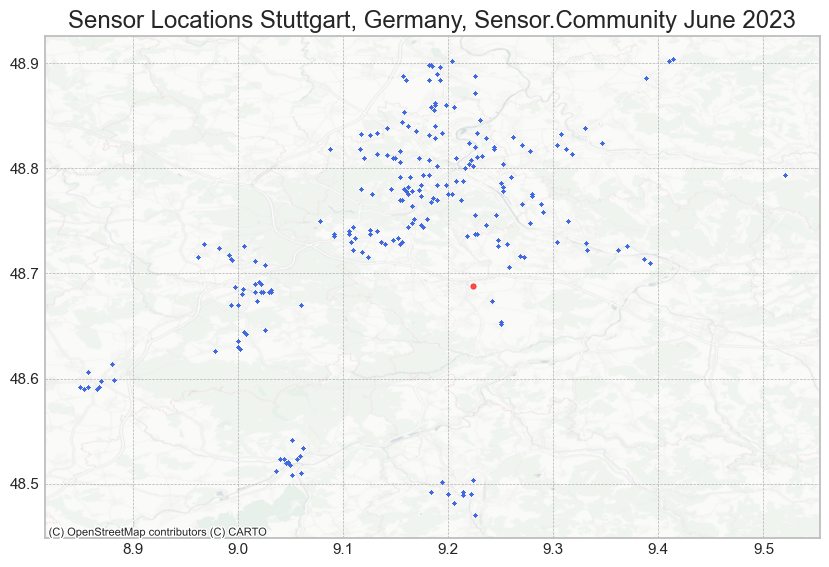
\includegraphics[width=1\textwidth]{images/sensor_community_locations_stuttgart_after_qc_june_23.png}
    \caption{Locations for Sensor.Community around Stuttgart, Germany, June 2023}
    \label{fig:qc sensor community stuttgart june 23}

    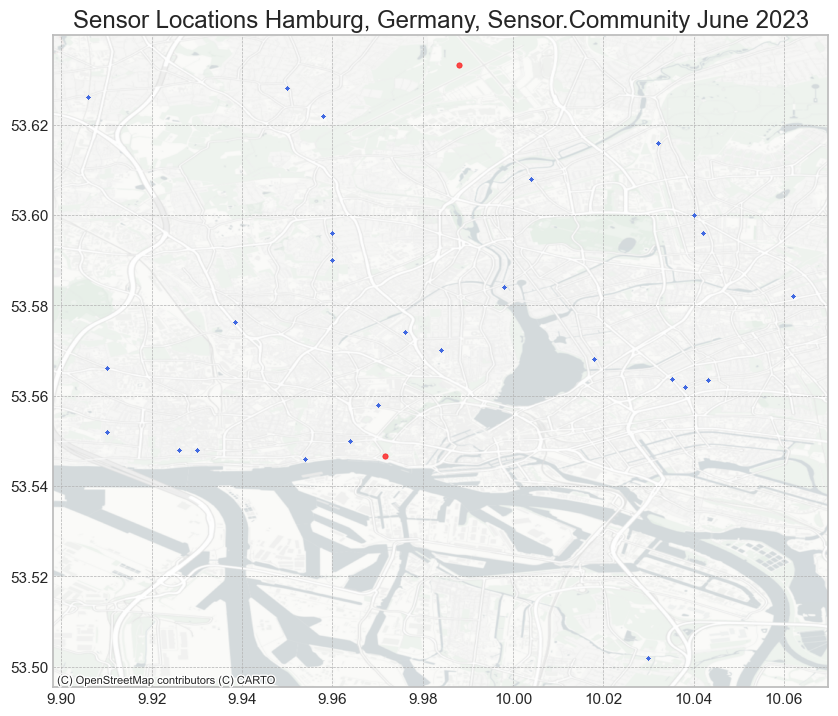
\includegraphics[width=1\textwidth]{images/sensor_community_locations_hamburg_after_qc_june_23.png}
    \caption{Locations for Sensor.Community in Hamburg, Germany, June 2023}
    \label{fig:qc sensor community hamburg june 23}
\end{figure}

- we choose stations from Stuttgart and Hamburg for the evaluation
-> identify stations with high mean daily temperature difference to reference station (to see if they are in a heat island)

\subsection{Stuttgart}

Station Locations:\\

\begin{figure}[ht]
    \centering
    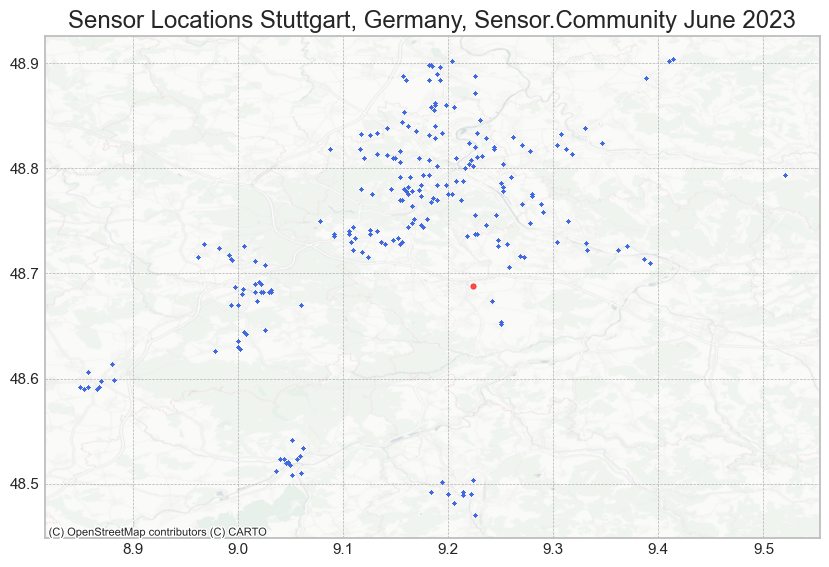
\includegraphics[width=1\textwidth]{images/sensor_community_locations_stuttgart_after_qc_june_23.png}
    \caption{Locations for Sensor.Community around Stuttgart, Germany, June 2023}
\end{figure}

DWD Reference location: 48.6883;9.2235 -> DWD id: 4931, Daily Max, Mean and Min values for June 2023\\

\begin{figure}[ht]
    \centering
    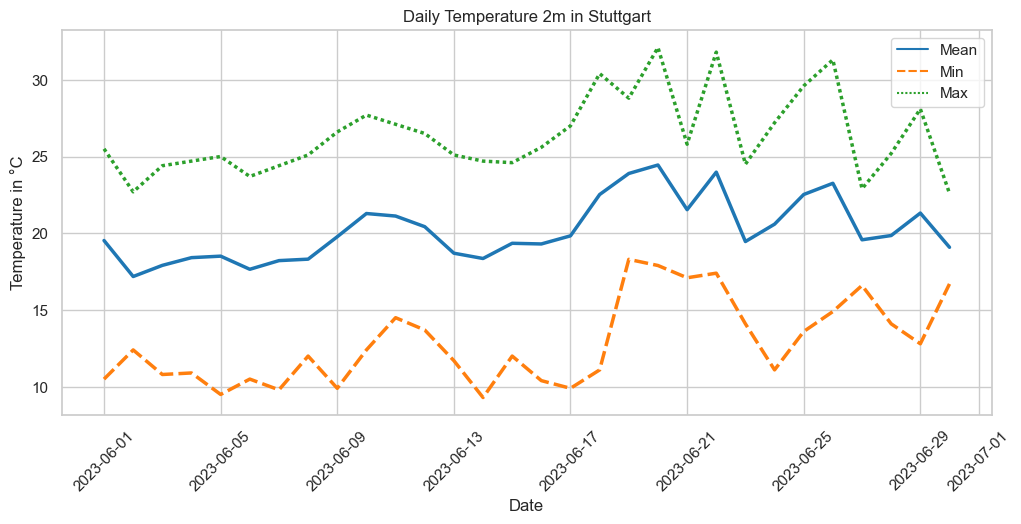
\includegraphics[width=1\textwidth]{images/dwd_stuttgart_june_23_tair_max_mean_min.png}
    \caption{Daily Mean, Max, and Min Air Temperature at 2m in Stuttgart, Germany, June 2023, DWD Station 4931}
    \label{fig:dwd mean max min stuttgart june 23}
\end{figure}


Steps:
- deterministic approaches
  - "naive" approach with nearest neighbor -> show high error rate
- probabilistic approaches
  - reference approach with geostatical methods (ordinary kriging, empirical bayesian kriging, EBK with regression) -> still high error rate, especially with lower density of weather stations/bad support for irregularly spaced data
    - ordinary krigin:
        - temperature semivariogram first
        - add additional features (e.g. soil temperature, land coverage, sky view factor, ...) as semivariograms and use cokrigin to combine them
    - empirical bayesian kriging:
        - not implemented out of the box (pykrige)

  - semivariogram: https://pro.arcgis.com/en/pro-app/latest/help/analysis/geostatistical-analyst/understanding-a-semivariogram-the-range-sill-and-nugget.htm

- deep learning approach with neural networks -> itteratively improve model by adding additional features, compare with reference approach

\section{Geostatical Interpolation Comparison}
In order to evaluate the performance of the ML model, we need to first get a better understanding of the interpolation quality of existing interpolation techniques. Next to simpler deterministic interpolation methods, such as inverse weight distance (IWD) or k-nearest neighbours (KNN) that are easy and performant, but struggle to capture more complex interdependencies, there are also more complex methods available. The most common geostatistical method for interpolation is Krigin, which is based on a gaussian process and uses a covariance function to model the spatial correlation between data points. The covariance function is a measure of the similarity between two data points, which is used to calculate the weight of the data point in the interpolation process. There are different types of Krigin methods available, each suited for different use cases, including:

\begin{enumerate}
    \item Simple Krigin: the simplest form of Krigin, that assumes that the mean of the measured values is known and constant
    \item Ordinary Krigin: same as Simple Krigin, but the mean is an unknown constant
    \item Universal Krigin: instead of assuming a constant mean, the mean is modeled as a deterministic function
    \item Indicator Krigin: same as Ordinary Krigin, but for categorical data
    \item Propability Krigin: same as Indicator Krigin, but assumes two types of random errors that can are each auto-correlated and cross-correlated to each other
    \item Disjunctive Krigin: same as Ordinary Krigin, but tries to improve the prediction quality by using an unknown constant and approximating an arbitrary function. It requires the bivariate normality assumption and is difficult to verify and solutions might be mathematically and computationally complicated
    \item Cokrigin: offers methods for the previous Krigin methods, but uses information on several variable types. This could improve the prediction quality, but might increase the variance of the prediction, as more much more estimation is required
\end{enumerate}

In the context of geostatistical analysis, there are different types of Krigin methods available that combine the aforementioned methods with other techniques, such as regression analysis. The following list is the geostaticial methods offered by ArcGIS Pro as part of the Geostatical Analyst toolbox~\footnote{\url{https://pro.arcgis.com/en/pro-app/latest/tool-reference/geostatistical-analyst/an-overview-of-the-geostatistical-analyst-toolbox.htm}}:

% TODO: add more details for each method
\begin{enumerate}
    \item Empirical Bayesian Krigin (EBK)
    \item Empircal Bayesian Krigin 3D (EBK3D)
    \item EBK Regression Prediction (EBKRP): Empirical Bayesian Kriging with regression prediction
    \item Global Polynominal Interpolation
    \item Kernel Interpolation with Barriers
    \item Moving Window Krigin
    \item Radial Basis Function
\end{enumerate}

In the scope of this work, we unfortunately cannot compare all of these methods with each other and therefore need to focus on a subset of methods. EBK and EBKRP are one of the most commonly used methods for temperature interpolation (cite). According to \cite{njoku2023effects}, EBKRP continously outperforms EBK in different weather station density scenarios, therefore we will use EBKRP as a baseline for our comparison.\\
In the following, the machine learning fundamentals for this work are explained and the different ML regression model types are introduced.

\section{Model Evaluation}

TODO

\subsection{Model Validity}

% TODO
Use 70\% of data for training, 30\% for test. cross-validation

\section{Variable Importance}

\section{Uncertainty Analysis}

measurement uncertainty, contextual uncertainty, prediction uncertainty

% Overall steps

1. Data Collection and rough analysis
  1.1. Get data from Sensor.Community
  1.2. Get data from DWD
  1.3. Get data from satellites via Google Earth Engine
  1.4. Get data from Netatmo (Hamburg, try to get Stuttgart as reference with historical data via API)
2. QC steps (TA first)
  2.1. Try to remove indoor stations and stations with irregular data
  2.2. Remove stations based on buddy check (removes a lot of sensor community stations due to lower density)
  2.3. Reference station has high quality data already, but can be used as a reference (interesting the comparison from 2m TA to 5cm TA)
  2.4. Discuss QA for other parameters (Humidity, Pressure etc.)
3. Comparison of models
  3.1. Simple models with only coordinates as input features and TA as target feature
  3.2. Add additional features (land coverage (NDVI, EVI)) and see how they improve the model
    3.2.1. For land coverage etc.\ compare different satellites and resolutions
    3.2.2. For coordinates/distances, compare different ways of calculating distances or modelling them in the model
    3.2.3. Compare influence of normalization
  3.3. Try to create a more complex NN model to show capabilities of NNs and try out LSTM for time series
  3.4. Choose final candidate that seems the most promissing and compare with reference approach
4. Comparison with refrence approaches
  4.1. Compare with simple Ordinary Kriging approach (with different kernels)
  4.2. Discuss problem of not being able to extrapolate

	% Summary
	\chapter{Conclusion}
\label{chap:Conclusion}
% 3 Pages

\section{Summary}

- discuss low amount of parameters and curse of dimensionality\\

TODO: Rewrite once Evaluation done\\
\\

With the growing need to analyze microclimates of cities in order to protect them against new phenomena like UHIs, this paper proposes the use of citizen-owned sensor networks that offer a higher spatial and temporal resolution of data points in comparison to traditional approaches such as relying on LST data. This approach also comes with challenges such as observing areas without stationary sensors and identifying poor quality data-points from broken or incorrectly installed sensors. With the obtained data, we create a temperature interpolation service that predicts temperature data between data points using a regression model that can act as a building block for further temperature-based analysis by abstracting the underlying single data-points in the data-layer away.\\
In order to improve the quality of temperature predictions for unobserved areas, we investigate how temporary sensor readings, f.e. by attaching sensors to buses, bikes or e-scooters, can be used to capture temporary local meteorological snapshots, and how these snapshots can be incorporated into the interpolation process. We also evaluate which features need to be captured to generate the most accurate predictions, if machine-learning is a suitable approach, and how it compares to more traditional geostatistical approaches.

\section{Future Outlook}

TODO
	\cleardoublepage
	
	% bibliography 
	\frontmatter
	\setcounter{page}{11}
	\bibliographystyle{alphadin}
	\bibliography{references}
	\cleardoublepage
	
	\appendix
	\chapter{Appendix}

\section{Netatmo}
\label{appendix: netatmo}

\begin{figure}[ht]
    \centering
    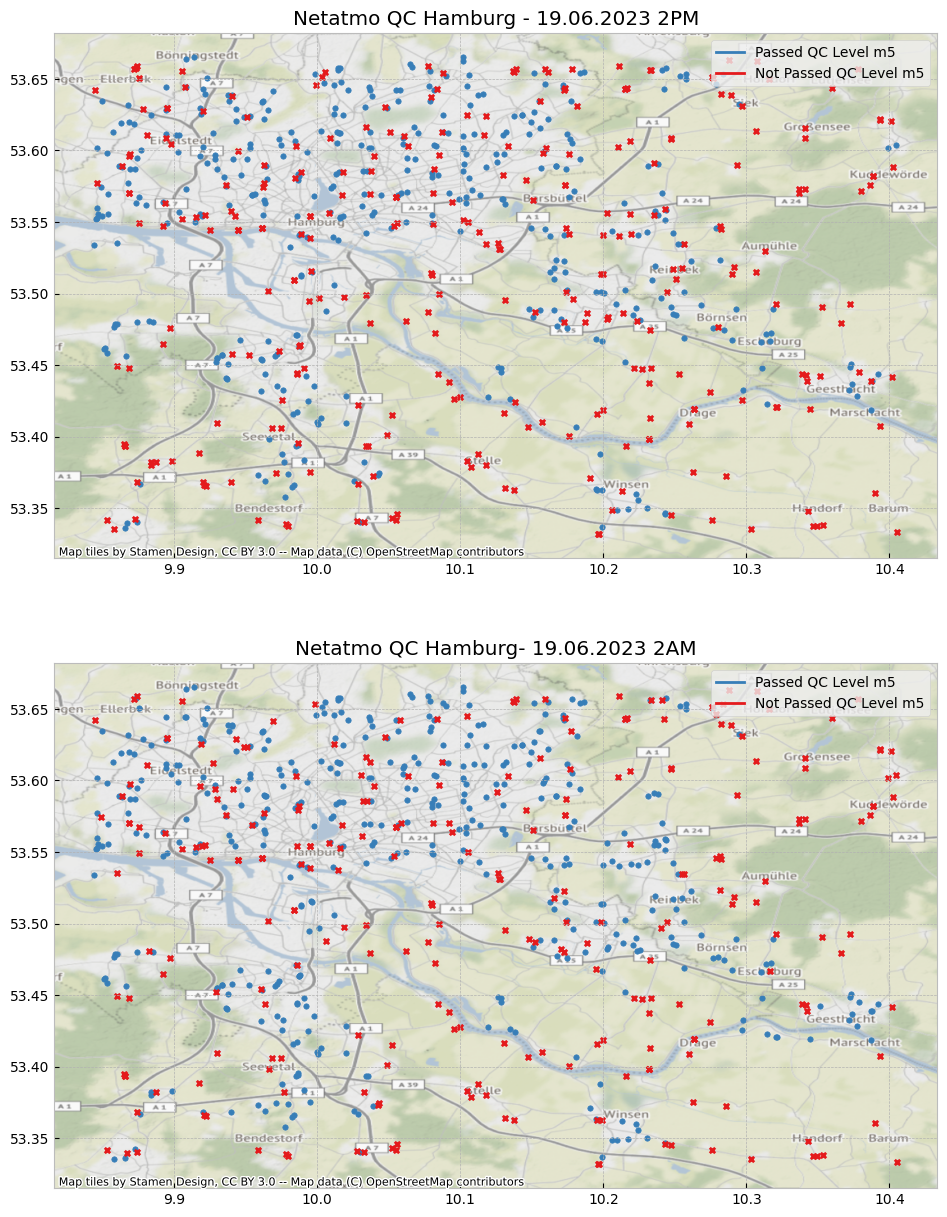
\includegraphics[width=.8\textwidth]{images/qc_hamburg_netatmo_june_before_after.png}
    \caption{\gls{qc} for Netatmo in Hamburg showing difference between day and night, 19.06.2023}
    \label{fig:qc netatmo hamburg before after m5}
\end{figure}

\begin{figure}[ht]
    \centering
    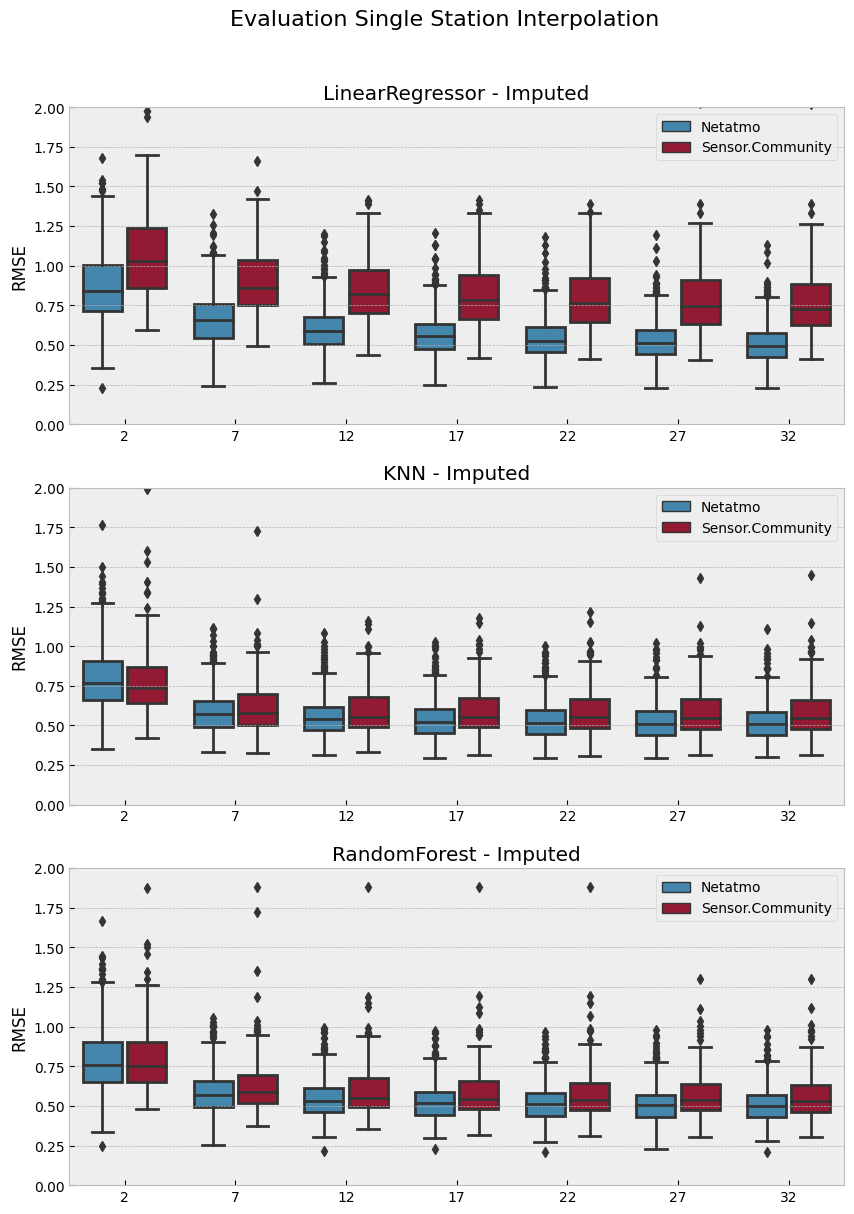
\includegraphics[width=0.9\textwidth]{images/eval imputed vs not imputed.png}
    \caption{Evaluation Single Station Interpolation, Detailed View}
    \label{fig:eval single station interpolation detailed}
\end{figure}

\begin{figure}[ht]
    \centering
    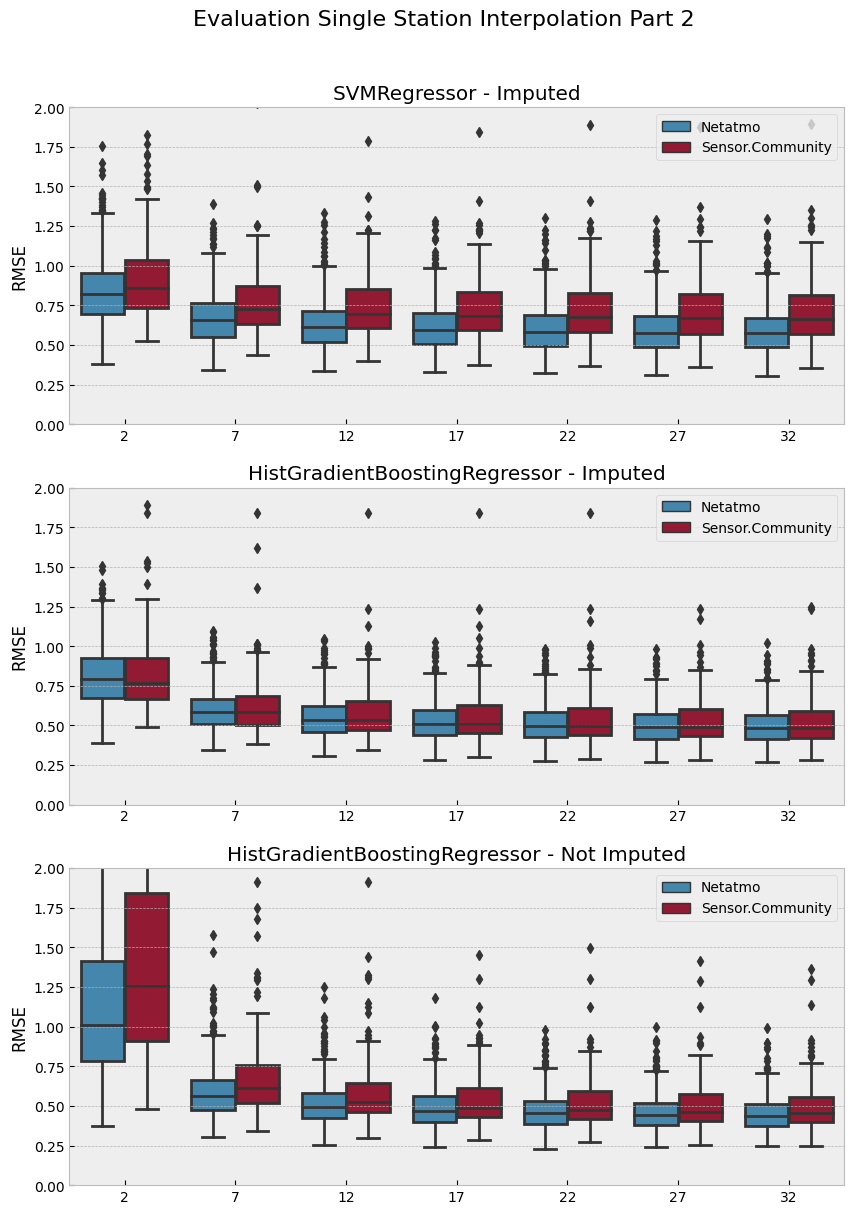
\includegraphics[width=0.9\textwidth]{images/eval imputed vs not imputed part 2.png}
    \caption{Evaluation Single Station Interpolation, Detailed View}
    \label{fig:eval single station interpolation detailed part 2}
\end{figure}

\section{Sklearn Model Parameters for Single Station Interpolation}
\label{appendix: sklearn ml parameters single station}

\begin{lstlisting}[language=Python, caption=Random Forest Regressor Parameters]
class sklearn.ensemble.RandomForestRegressor(n_estimators=200,
*, criterion='squared_error', max_depth=None, min_samples_split=2,
min_samples_leaf=1, min_weight_fraction_leaf=0.0, max_features=1.0,
max_leaf_nodes=None, min_impurity_decrease=0.0, bootstrap=True,
oob_score=False, n_jobs=None, random_state=None, verbose=0,
warm_start=False, ccp_alpha=0.0, max_samples=None)
\end{lstlisting}

The number of trees was increaed from 100 to 200 to increase the performance.

\begin{lstlisting}[language=Python, caption=Histogram-based Gradient Boosting Parameters]
class sklearn.ensemble.HistGradientBoostingRegressor
(loss='squared_error', *, quantile=None, learning_rate=0.1,
max_iter=200, max_leaf_nodes=31, max_depth=None, min_samples_leaf=20,
l2_regularization=0.0, max_bins=255, categorical_features=None,
monotonic_cst=None, interaction_cst=None, warm_start=False,
early_stopping='auto', scoring='loss', validation_fraction=0.1,
n_iter_no_change=10, tol=1e-07, verbose=0, random_state=42)
\end{lstlisting}

The number of max iterations was increased from the default value of 100 to 200 to improve the performance of the model and the random state was set to 42 so all interations yield the same result.

\section{Feature Engineering}

\begin{lstlisting}[language=Python, caption=Timestamp to Sinus Curve Feature, label=lst: timestamp to sin]
    # Convert datetime64 timestamp hours and minutes to circle angle
    filtered_gdf['time'] = filtered_gdf['time'].apply(lambda x: (x.hour * 60 + x.minute) * 2 * np.pi / (24 * 60))
    filtered_gdf.rename(columns={'time': 'time_angle'}, inplace=True)

    # Calculate continuous representation of time as an angle in radians
    filtered_gdf['sin_time'] = np.sin(filtered_gdf['time_angle'])
\end{lstlisting}

\section{Histogram-based Gradient Boosting Single Location Interpolation}

\subsubsection{List of stations for minimum distance between stations}
\label{appendix stations for minimum distance between stations}

The list of stations for the minimum distance between stations is the following by their Netatmo station id:

\begin{itemize}
    \item 70:ee:50:83:b1:e2 
    \item 70:ee:50:16:16:ce
    \item 70:ee:50:5e:d4:16
    \item 70:ee:50:00:d3:96
    \item 70:ee:50:6b:5f:50
    \item 70:ee:50:00:d1:1c
    \item 70:ee:50:5f:51:a0
    \item 70:ee:50:6b:97:86
    \item 70:ee:50:28:f2:ca
    \item 70:ee:50:58:e8:70
\end{itemize}

The locations of the stations are presented in Figure~\ref{fig:eval_hamburg_locations_point_histb_10_map}.

\begin{figure}[ht]
    \centering
    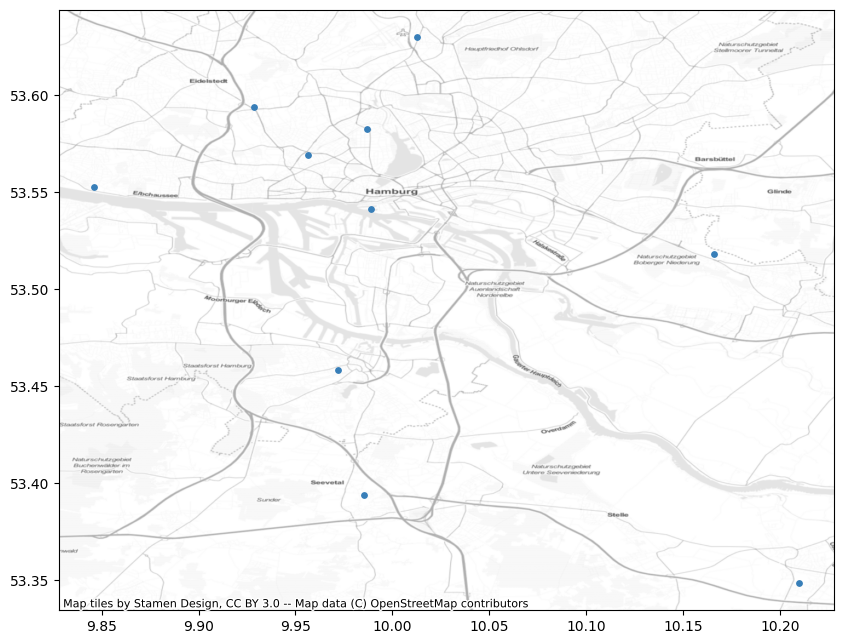
\includegraphics[width=1\textwidth]{images/eval_hamburg_locations_point_histb_10_map.png}
    \caption{Netatmo Stations for Minimum Distance Between Stations, Hamburg}
    \label{fig:eval_hamburg_locations_point_histb_10_map}
\end{figure}

\section{Areal Interpolation}

Figure~\ref{fig:dwd stuttgart june 23 mean min max} shows the mean/max/min \gls{ta} for \gls{dwd} station with id 4931 across June 2023 in Stuttgart near the airport.
Figure~\ref{fig:dwd stuttgart june 23 10 min 2m 5cm} shows the \gls{ta} for the same station on the 19. June 2023 in a 10 minute interval. The blue line, i.e., TT\_10, shows the \gls{ta} at 2m while the orange line, i.e., TM5\_10, shows the \gls{ta} at 5cm directly above the ground.

\begin{figure}[ht]
    \centering
    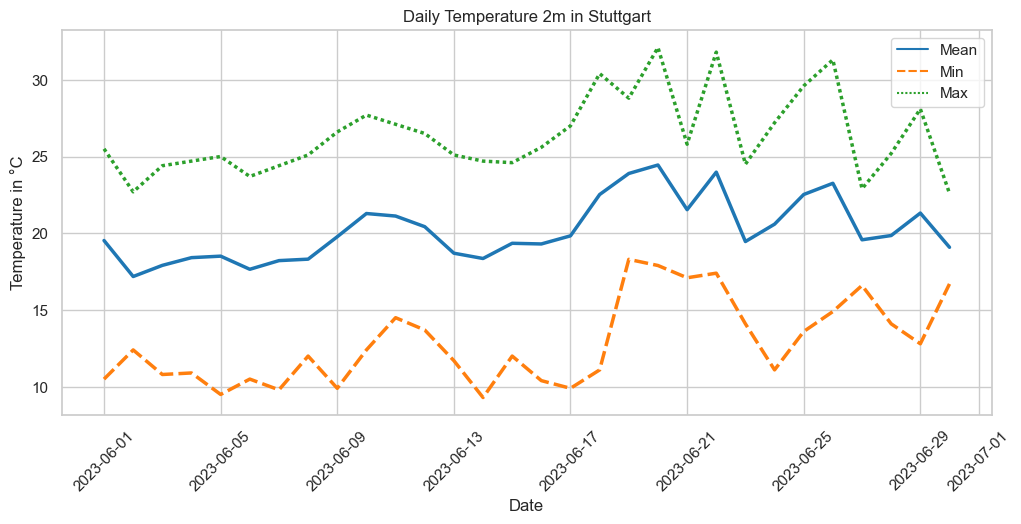
\includegraphics[width=1\textwidth]{images/dwd_stuttgart_june_23_tair_max_mean_min.png}
    \caption{\gls{dwd} Station 4931, Stuttgart, June 2023}
    \label{fig:dwd stuttgart june 23 mean min max}

    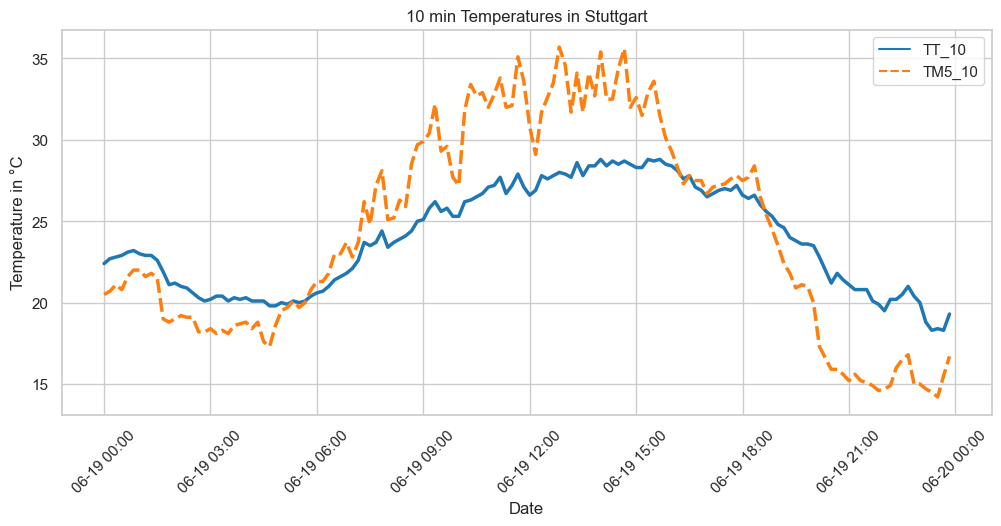
\includegraphics[width=1\textwidth]{images/dwd_stuttgart_june_19_23_tair.png}
    \caption{\gls{dwd} Station 4931, Stuttgart, 19. June 2023}
    \label{fig:dwd stuttgart june 23 10 min 2m 5cm}
\end{figure}

	\section{Sensor Community}

\lstinputlisting[language=C,caption=Sensor Distribution by Country,label=sensor_community_sensors_by_countries]{appendix/sensor_community_sensor_countries.json}

	% affidavit
		\chapter*{Eidesstattliche Versicherung}
\renewcommand*\chapterpagestyle{empty}
\addcontentsline{toc}{chapter}{Eidesstattliche Versicherung}
Hiermit versichere ich an Eides statt, dass ich die vorliegende Arbeit im Studiengang XXX %TODO Studiengang anpassen
selbstständig verfasst und keine anderen als die angegebenen Hilfsmittel – insbesondere keine im Quellenverzeichnis nicht benannten Internet-Quellen – benutzt habe.
Alle Stellen, die wörtlich oder sinngemäß aus Veröffentlichungen entnommen wurden, sind als solche kenntlich gemacht. 
Ich versichere weiterhin, dass ich die Arbeit vorher nicht in einem anderen Prüfungsverfahren eingereicht habe und die eingereichte schriftliche Fassung der auf dem elektronischen Speichermedium entspricht.
\vspace{1cm} 

\noindent Hamburg, den \uline{~~~~~~~~~~~~~~~~~~~~~~~~~~~~~~~}~~~~~~~Unterschrift: \uline{~~~~~~~~~~~~~~~~~~~~~~~~~~~~~~~~~~~~~~~~~~~~~~~~~~} 

\let \cleardoublepage \clearpage

\noindent\begin{minipage}{\textwidth}
	
\vspace{1cm} 
\chapter*{Veröffentlichung}
Ich stimme der Einstellung der Arbeit in die Bibliothek des Fachbereichs Informatik \\zu.
\vspace{1cm}\\ 
\noindent Hamburg, den \uline{~~~~~~~~~~~~~~~~~~~~~~~~~~~~~~~}~~~~~~~Unterschrift: \uline{~~~~~~~~~~~~~~~~~~~~~~~~~~~~~~~~~~~~~~~~~~~~~~~~~~}
\end{minipage}

	
\end{document}